\documentclass[11pt]{caltech_thesis} % font size must be changed in the caltech_thesis.cls file. 
% [11pt] has no effect here
\usepackage[hyphens]{url}
\usepackage{lipsum}
\usepackage{graphicx}
\usepackage{todonotes}
\usepackage[utf8]{inputenc}
\usepackage[T1]{fontenc}
\usepackage{mathpazo}
\usepackage[numbers,sort&compress]{natbib}
\usepackage{csquotes}
\usepackage{bibunits}
\usepackage{enumitem}
\usepackage{amsmath}
\usepackage{longtable}
\usepackage{xcolor} 
\usepackage{indentfirst} 
\usepackage{microtype} 
\usepackage{upgreek} % for non-italic greek letters (units)
\usepackage[outputdir=../]{minted} % for code highlighting
\definecolor{CaltechOrange}{HTML}{FF6C0C}
\definecolor{midnightblue}{HTML}{3F3F9E}
\definecolor{darkred}{HTML}{BA1A1A}
\definecolor{extralightgray}{HTML}{F5F5F5}
\usepackage[hidelinks=true,
            colorlinks=true, 
            linkcolor=black,
            urlcolor=CaltechOrange, 
            linkbordercolor=white,
            backref=false,
            pagebackref=false,
            hyperindex=false,
            breaklinks=true,
            bookmarks=false,
            bookmarksopen=false,
            ]{hyperref}
\usepackage[
            backend=biber,natbib,
            % IMPORTANT: load a style suitable for your discipline
            style=ieee
        ]{biblatex}


% added to conform with this issue: https://github.com/jgm/pandoc/issues/4384
% with this, figure width can be changed with {width: 70%}
\makeatletter
\def\maxwidth{\ifdim\Gin@nat@width>\linewidth\linewidth\else\Gin@nat@width\fi}
\def\maxheight{\ifdim\Gin@nat@height>\textheight\textheight\else\Gin@nat@height\fi}
\makeatother
% Scale images if necessary, so that they will not overflow the page
% margins by default, and it is still possible to overwrite the defaults
% using explicit options in \includegraphics[width, height, ...]{}
\setkeys{Gin}{width=\maxwidth,height=\maxheight,keepaspectratio}

\hypersetup{
  colorlinks = true,
  linkcolor = black
}

\makeatletter
\let\@mycite\@cite
\def\@cite#1#2{{\hypersetup{linkcolor=black!60!black}[{#1\if@tempswa , #2\fi}]}}
\makeatother
            
\addbibresource{references_cleaned.bib}
\defaultbibliographystyle{plainnat}
\renewcommand{\bibsection}{\section*{\refname}}
\usepackage{memhfixc}
\linespread{1.5}


\begin{document}

\title{Precise Quantum Measurements with Superconducting Nanowire Single Photon Detectors}
\author{Andrew Sterling Mueller}
\degreeaward{Doctor of Philosophy in Applied Physics}                 
\university{California Institute of Technology}    
\address{Pasadena, California}                     
\unilogo{caltech.png}                                 
\copyyear{2024}  
\defenddate{December 2023}   
       
\orcid{0000-0002-6598-9732}



\rightsstatement{Some rights reserved. This thesis is distributed under a
Creative Commons Attribution License CC-BY 4.0. All software used in the
analysis and generation of figures is distributed under an MIT license, and
is available on a GitHub repository
\href{https://github.com/sansseriff/phd_thesis}{https://github.com/sansseriff/phd\textunderscore thesis}}

\maketitle[logo]

\begin{acknowledgements}   
    \input{frontmatter/acknowledgements.md}
\end{acknowledgements}

\begin{abstract}
  \input{frontmatter/abstract.md} 
\end{abstract}

\extrachapter{Published Content and Contributions}
\begin{publishedcontent}
\input{frontmatter/published.md}
\end{publishedcontent}

\tableofcontents
\listoffigures
\listoftables
\printnomenclature
\mainmatter

\hypertarget{introduction}{%
\chapter{Introduction}\label{introduction}}

background of snspds here. current capabilities and operation principle. New stuff.

About the differential single pixel here

structure of this thesis here

\hypertarget{low-dark-count-rate-detection}{%
\chapter{Low Dark Count Rate Detection}\label{low-dark-count-rate-detection}}

The work described in this chapter culminated in the research paper: Andrew S. Mueller, Boris Korzh, Marcus Runyan, Emma E. Wollman, Andrew D. Beyer, Jason P. Allmaras, Angel E. Velasco, Ioana Craiciu, Bruce Bumble, Ryan M. Briggs, Lautaro Narvaez, Cristián Peña, Maria Spiropulu, and Matthew D. Shaw, ``Free-space coupled superconducting nanowire single-photon detector with low dark counts,'' \href{https://opg.optica.org/optica/fulltext.cfm?uri=optica-8-12-1586\&id=465726}{Optica 8, 1586-1587 (2021)}

Boriz Korzh provided extensive assistance during ideation, construction, testing, and copyediting phases of the experiment. Bruce Bumble designed the elevated 0.8 K stage and innovated translation system using flexible carbon fiber rods. Jason Trevor provided technical assistance with the implementation of a nitrogen flow bag. Sahil Patel assisted with editing the manuscript.

\hypertarget{abstract}{%
\section{Abstract}\label{abstract}}

\emph{A free-space coupled superconducting nanowire single photon detector with high efficiency at 1550 nm, sub-0.1 Hz dark count rate, and sub-15 ps timing jitter is demonstrated.}

\hypertarget{background}{%
\subsubsection{Background}\label{background}}

Superconducting nanowire single photon detectors are high sensitive devices. Any stray photons from a laboratory environment can make their way into these devices and produce a detection. These detections are commonly called dark counts or false counts. Dark counts can be present in any situation where the detector is coupled to some experiment or apparatus outside the cryogenic environment. This coupling may be through windows inside the cryostat housing and radiations shields, or through optical fibers that carry single-mode signals directly to detectors.

Visible, near-infrared, and mid-infrared photons are often the main sources of dark counts, because they are ubiquitous in a laboratory environment and are transmitted through common types of fibers and windows. Assuming visible light can be blocked from entering the detector system, the blackbody emission of the room temperature laboratory environment presents is the primary source of dark counts. The spectrum of blackbody photons, defined by Planck's law, is peaked at about $10~\mathrm{\upmu m}$, though it can contribute dark counts at significant rates up through near-infrared wavelengths.

Without filtering in fiber or free space, dark counts from blackbody emission will overload most SNSPDs and overpower the extremely faint signal of interest.

\hypertarget{introduction-1}{%
\section{Introduction}\label{introduction-1}}

Time-resolved photon detection with low dark counts is a vital technology in fields such as quantum information processing, classical communication, quantum communication, and laser ranging. Increasingly, research in these fields employs superconducting nanowire single photon detectors (SNSPDs), which have been demonstrated with system detection efficiency ($\eta$) of more than 90\% \autocite{Reddy2020}, timing jitter ($\Delta t$) as low as 2.6 ps \autocite{Korzh2020} and intrinsic dark count rates ($D$) in the milli- to micro-hertz range \autocite{Hochberg2019}. However, quantum communication applications require detection systems with performance optimized across all three metrics simultaneously. The dimensionless figure of merit $H$ specifies this application-specific performance as $H = \frac{\eta}{(\Delta t D)}$~\autocite{Hadfield2009}.

Here, we focus on lowering the Dark Count Rate (DCR) of a telecom-band SNSPD system by filtering thermal photons, without sacrificing efficiency or jitter. We demonstrate a free-space coupled SNSPD with sub-0.1 Hz DCR, 14 ps timing jitter, and 72\% total system detection efficiency (SDE) by using a differential single-pixel SNSPD \autocite{Colangelo2021} to image a single-mode fiber through an optimized free-space filter stack.

The highest system detection efficiencies have been achieved using self-aligned fiber coupling where dark counts can be reduced using cryogenic fiber looping \autocite{Cohen2015} or spliced narrow-band filters \autocite{Boaron2018secure}. But it is difficult to achieve strong filtering without losses at the target wavelength. Low-loss, high-rejection filters are typically available as free-space components, so some of the highest reported H-values were achieved with cryogenic, fiber to free-space to fiber coupling, but exhibit an SDE of only a few percent \autocite{Shibata2015}. The filtering method presented here takes advantage of commercially-available filters, achieves a high free-space coupling efficiency using a cryogenic lens, and is compatible with both fiber and free-space optical inputs.

In this work, a single mode fiber is imaged onto the detector using two f = 18.75 mm lenses. One lens collimates light from an optical fiber face outside the cryostat (Photon Spot), and the other focuses light onto the detector inside \autocite{Bellei:16}. In the collimated region between, the beam passes though a series of short-pass filters and one band-pass filter mounted at 4 K (Fig. \ref{fig:setup}a). One of the short-pass filters is angled to avoid ghosting effects. The 40 K radiation shield and outer cryostat housing are fitted with anti-reflection coated BK7 windows. The filters are spring loaded to prevent cracking at low temperatures. To minimize effects of stray light, the interior of the 4 K shield was painted with mid-IR absorbing paint (Aeroglaze Z306) \autocite{Persky1999}, while gaps between filters and the windows were covered with metal tape.

The system is based on 1-inch optics, although the f = 18.75 mm lenses lead to a $1/e^2$ intensity diameter of about 5 mm in the collimated region. To reduce the larger-than-required numerical aperture of the system, painted 8 mm apertures (Acktar Spectral Black) were added in the collimated region. These are large enough to allow minor alignment adjustments --- by translating the exterior collimating lens --- without vignetting.

\hypertarget{fig:dcrmin_data}{%
\begin{figure}
\centering
\includegraphics{./chapter_02/figs/DataFigure_6.svg}
\caption[{Low Dark Count Rate Project Results.}]{\textbf{Low Dark Count Rate Project Results} a) Simulated photon flux at various temperatures with and without the 1550 nm bandpass filter (BP). b) Normalized photon count rate (PCR) and jitter measurements c) DCR, and calculated figure of merit $H$ versus bias current for both fiber-coupled and free space coupled configurations.}
\label{fig:dcrmin_data}
\end{figure}
}

We use four custom cryogenic short-pass filters, with pass-bands below $1.6 \ \mathrm{\upmu m}$ and $1.9 \ \mathrm{\upmu m}$ (Andover Corp.), both with transmission at 1550 nm of 98.8 ± 0.3\%. They reject wavelengths shorter than $3 \ \mathrm{\upmu m}$ through reflective optical coatings, and attenuate longer wavelengths through material absorption in the 12.7 mm-thick N-BK7 glass substrate. While the bandpass filter (FWHM = 7 nm) was found to blue-shift by about 2 nm at cryogenic temperatures, the passband was wide enough such that significant attenuation was not observed at the original target wavelength of 1550 nm. This filter is also sufficiently wide to avoid Fourier-limited broadening of ultra-short laser pulses.

The filtering of the optical stack was modeled by assuming a black-body emitter at 298 K and a field of view defined by the 18.75 mm focal length of the cryogenic lens and the 8 mm diameter of the apertures. The resulting spectrum was multiplied by the transmission of the filters (Fig. \ref{fig:setup}b) and detector optical stack (Fig. \ref{fig:setup}c). The model showed that two each of the $1.6 \ \mathrm{\upmu m}$ and $1.9 \ \mathrm{\upmu m}$ short pass filters were necessary to suppress mid-infrared light to where it was no longer the dominant source of dark counts. With the inclusion of the four shortpass filters, the dominant source of dark counts is the spectral region near 1550 nm as shown in Fig. \ref{fig:false-color}a, which also illustrates the effect of the bandpass filter. Also evident in Fig. \ref{fig:false-color}a is the strong dependence of DCR on the temperature of the final surface outside the cryostat emitting thermal radiation. This motivated the exterior cooling apparatus shown at the bottom of Fig. \ref{fig:setup}a. The bulkhead holding the fiber connector is cooled to around -2$^\circ$C using a Peltier element and liquid cooling block. This addition reduced the system DCR from 0.4 Hz to below 0.1 Hz. While dark counts from multiple spatial modes are present in this system --- modes that would not be present in a purely fiber based approach --- the external cooling technique works to minimize their effect.

This work used a low-jitter, differential SNSPD \cite{Colangelo2021}, with an active area of $22 \times 15 \ \mathrm{\upmu m}$, formed by a meander of 100 nm-wide and 5-nm-thick niobium nitride (NbN) nanowires on a 500 nm pitch. A more conventional single-ended readout SNSPD of similar area would also achieve low DCR in this coupling system, but would likely achieve a lower performance metric $H$ from correspondingly higher jitter. The nanowire is embedded in an efficiency-enhancing optical stack made of alternating layers of TiO$_2$ and SiO$_2$ and a gold mirror layer. As shown in Fig. \ref{fig:false-color}b and c, when fiber coupled (without any fiber-based filtering methods applied), this detector achieved a saturated SDE of $84\% \pm 4.4 \%$ and a DCR of 20 Hz at a bias current of $16\ \mathrm{\upmu A}$.

~~~~~ As also shown in Fig. \ref{fig:false-color}b, the free-space coupling system achieves up to $72 \% \pm 3.7 \%$ SDE as measured from the fiber outside the cryostat. The reduction in efficiency is likely due to surface reflections in the free-space optics, and potential misalignment in the optical baffles. The minimum DCR (Fig. \ref{fig:false-color}c) at $72 \%$ SDE is about 0.1 Hz, with a bias current of 16 $\mathrm{\upmu A}$. These metrics, with the jitter measurements shown in Fig. \ref{fig:false-color}b, give a maximum H value of $5 \times 10^{11}$ (Fig. \ref{fig:false-color}c). Values as high as $1.8 \times 10^{12}$ have been reported before, but at 1.5\% system detection efficiency \cite{Shibata2015}. Our system shows a low DCR can be achieved without severe reduction of SDE or usable target wavelength bandwidth. This is paramount for the future of terrestrial and space-to-ground quantum communication, since it increases success rate with finite statistics \cite{Boaron2018secure}. The same techniques can be applied to emerging SNSPD applications at longer wavelengths, such as laser ranging \cite{Taylor2019}, where fiber filtering is impractical. Beyond single-mode applications, our work paves the way to scalable, low-DCR, multi-mode coupling to SNSPD arrays \cite{Wollman2019}.

\hypertarget{fig:custom_figure}{%
\begin{figure}
\centering
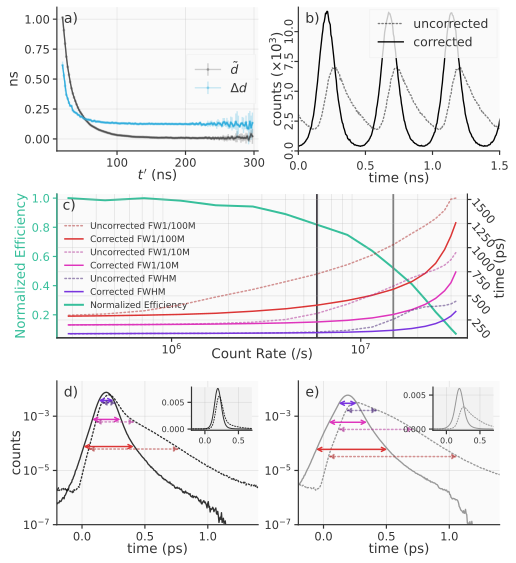
\includegraphics[width=0.7\textwidth,height=\textheight]{./chapter_02/figs/Figure_Data_Sept_2022_light.svg}
\caption[{A jitterate data figure.}]{\textbf{Figure Title.} And I think the rest of this is the caption with (A), (B), and (C) callouts}
\label{fig:custom_figure}
\end{figure}
}

Finally, here's a png figure for testing

\hypertarget{fig:test_png_figure}{%
\begin{figure}
\centering
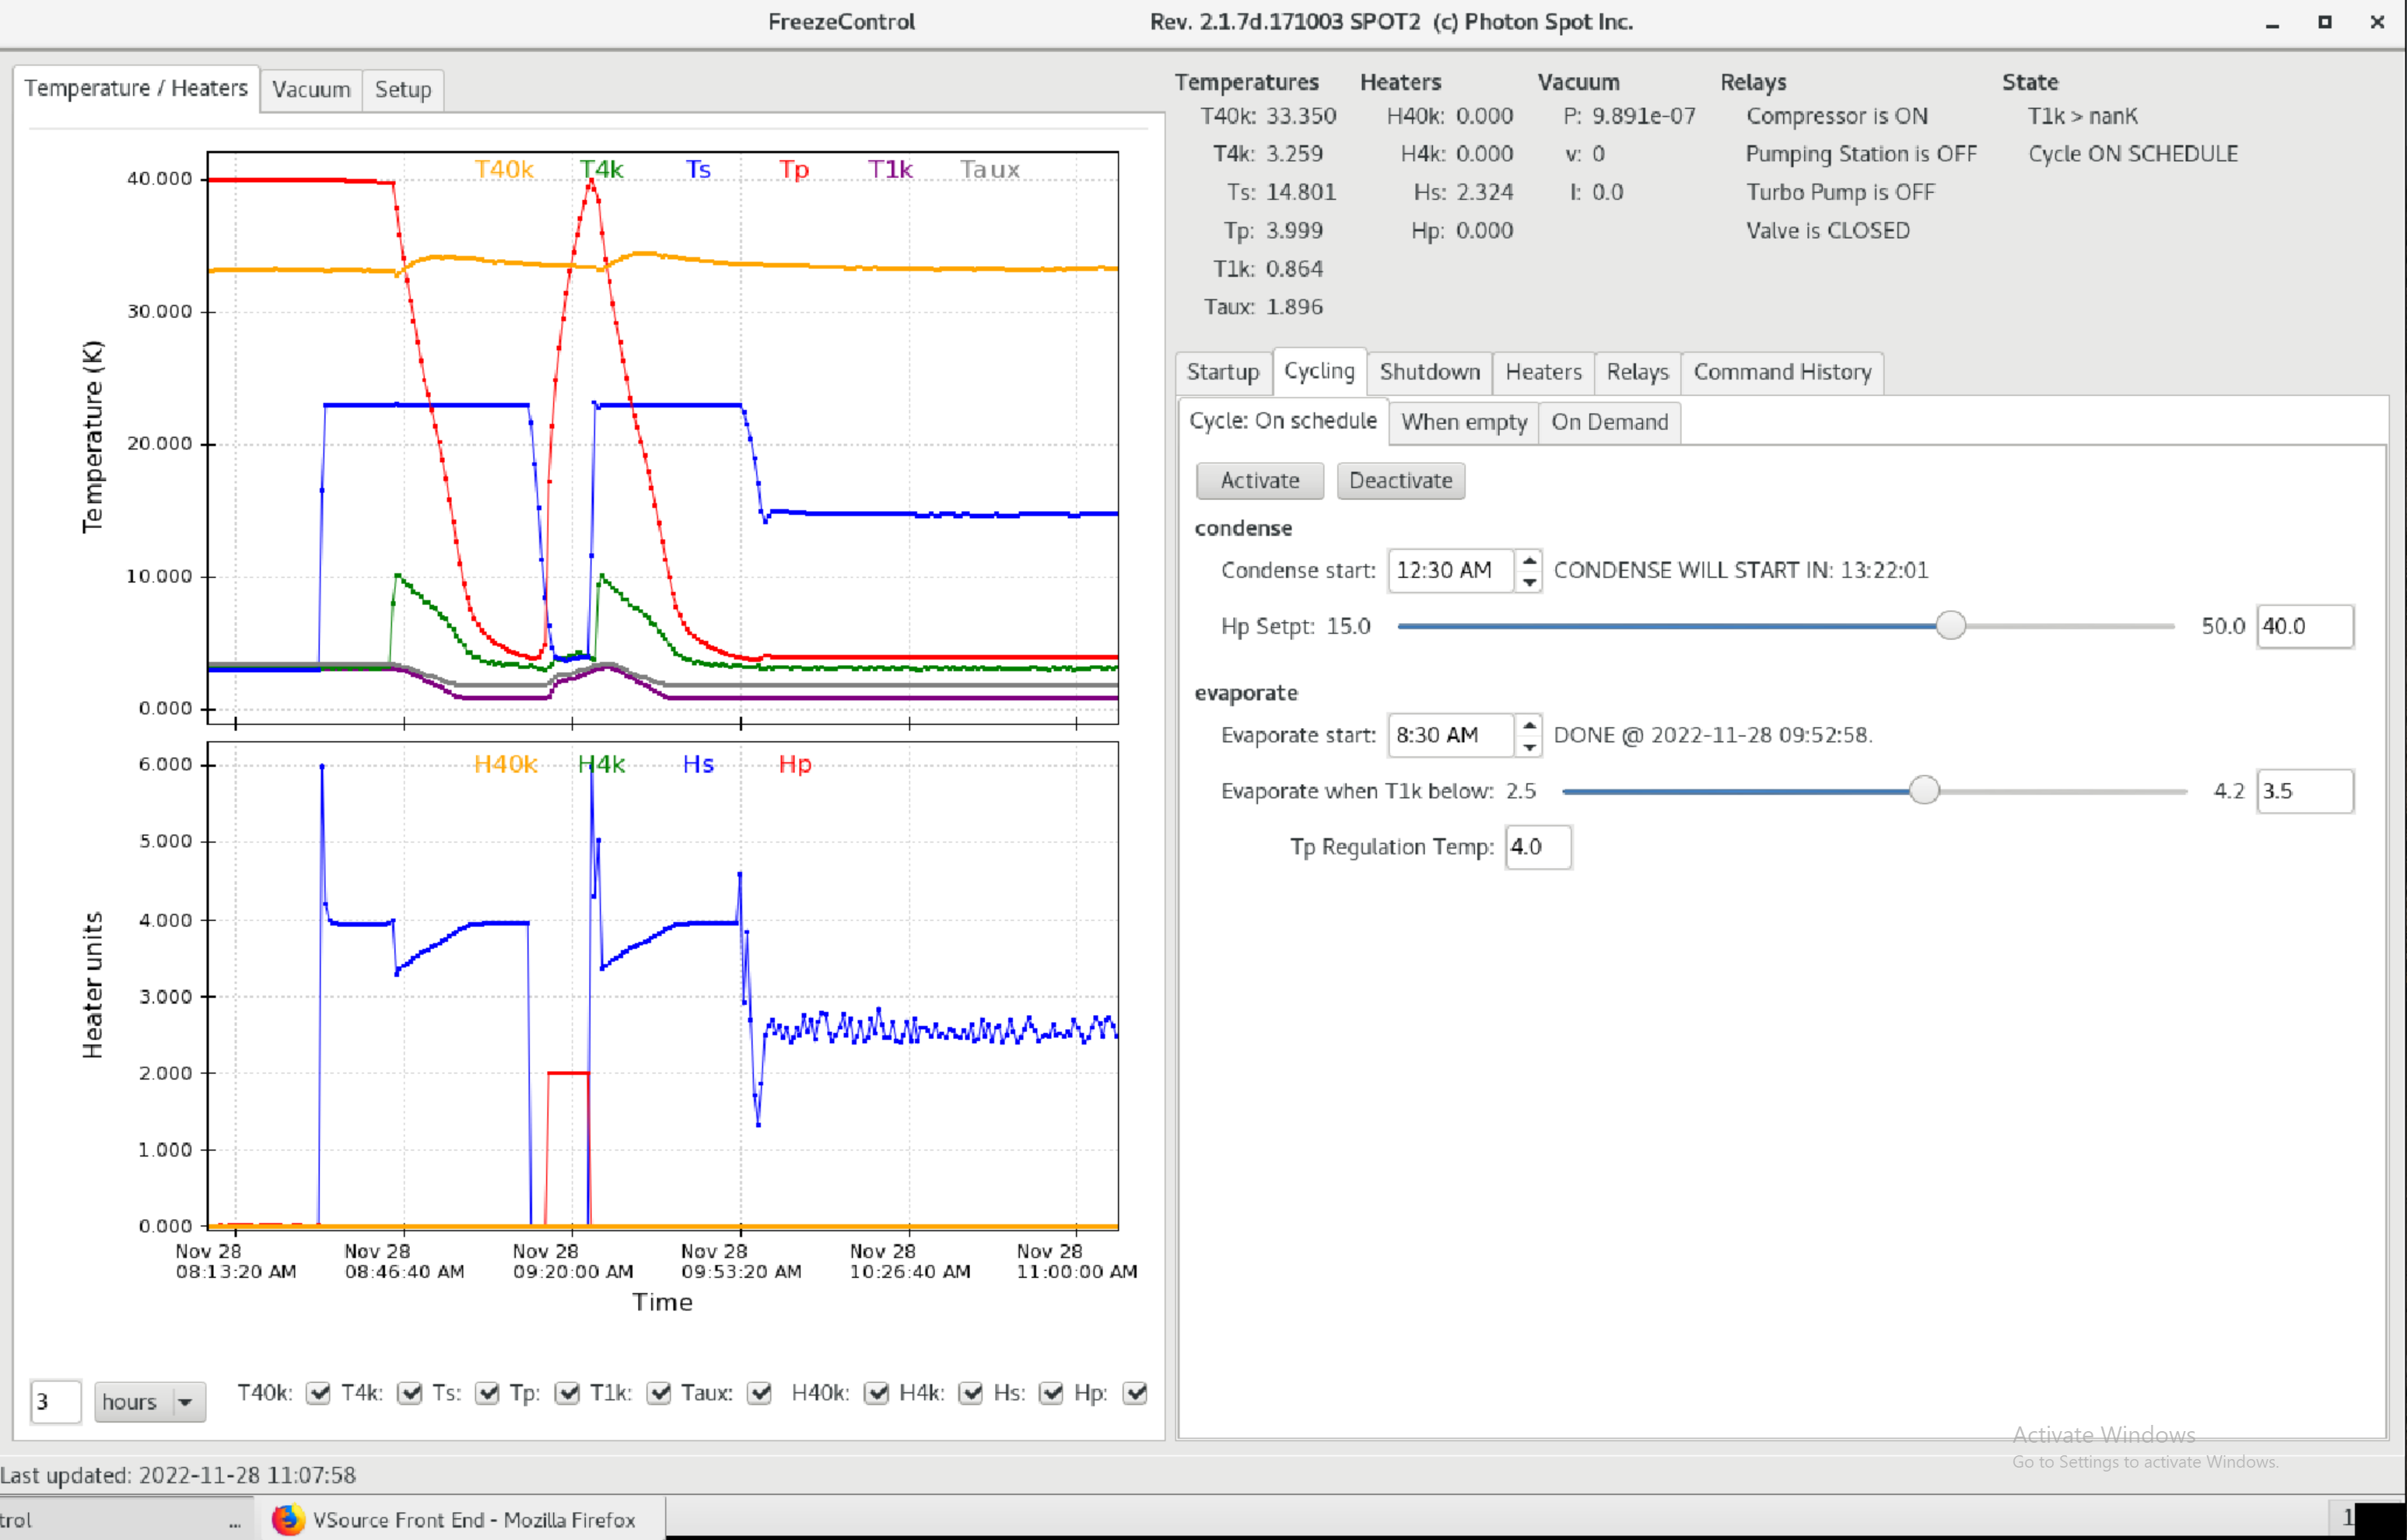
\includegraphics[width=0.7\textwidth,height=\textheight]{./chapter_02/figs/fridge.png}
\caption[{A png figure.}]{\textbf{A test png figure.} And here is where I'd put in more information about the png.}
\label{fig:test_png_figure}
\end{figure}
}

Remember there's a lot of optics stuff you got good at, like how to focus a spot inside the fridge using only optics outside the fridge. How you used the xyz stage on the fiber for that, and the xy or the mirror. How you defocused the laser to see the detector when you were using the narroband filter.

\hypertarget{time-walk-and-jitter-correction}{%
\chapter{Time Walk and Jitter Correction}\label{time-walk-and-jitter-correction}}

A version of this chapter is currently published as:

Andrew Mueller, Emma E. Wollman, Boris Korzh, Andrew D. Beyer, Lautaro Narvaez, Ryan Rogalin, Maria Spiropulu, Matthew D. Shaw; \href{https://pubs.aip.org/aip/apl/article/122/4/044001/2870246/Time-walk-and-jitter-correction-in-SNSPDs-at-high}{Time-walk and jitter correction in SNSPDs at high count rates}. Appl. Phys. Lett. 23 January 2023; 122 (4): 044001.

Portions of this chapter appear in:

Ioana Craiciu, Boris Korzh, Andrew D. Beyer, Andrew Mueller, Jason P. Allmaras, Lautaro Narváez, Maria Spiropulu, Bruce Bumble, Thomas Lehner, Emma E. Wollman, \& Matthew D. Shaw (2023). \href{https://opg.optica.org/optica/fulltext.cfm?uri=optica-10-2-183\&id=525546}{High-speed detection of 1550 nm single photons with superconducting nanowire detectors}. Optica, 10(2), 183--190.

\hypertarget{abstract-1}{%
\section{Abstract}\label{abstract-1}}

~~~~~

Superconducting nanowire single-photon detectors (SNSPDs) are a leading detector type for time correlated single photon counting, especially in the near-infrared. When operated at high count rates, SNSPDs exhibit increased timing jitter caused by internal device properties and features of the RF amplification chain. Variations in RF pulse height and shape lead to variations in the latency of timing measurements. To compensate for this, we demonstrate a calibration method that correlates delays in detection events with the time elapsed between pulses. The increase in jitter at high rates can be largely canceled in software by applying corrections derived from the calibration process. We demonstrate our method with a single-pixel tungsten silicide SNSPD and show it decreases high count rate jitter. The technique is especially effective at removing a long tail that appears in the instrument response function at high count rates. At a count rate of 11.4 MCounts/s, we reduce the full width at 1\% maximum level (FW1\%M) by 45\%. The method, therefore, enables certain quantum communication protocols that are rate-limited by the FW1\%M metric to operate almost twice as fast.

\hypertarget{introduction-2}{%
\section{Introduction}\label{introduction-2}}

\hypertarget{origin-of-time-walk}{%
\subsection{Origin of time walk}\label{origin-of-time-walk}}

Over the last decade, SNSPDs have advanced rapidly to become essential components in many optical systems and technologies, owing to their high efficiency $(>90\%)$~\autocite{99.5_Chang_2021,reddy2020superconducting}, fast reset times ($< 1~\mathrm{ns}$)~\autocite{Vetter2016Cavity} and scalability to kilopixel arrays~\autocite{Wollman2019}. The timing jitter of SNSPDs is also best-in-class -- values as low as 3~ps have been demonstrated in short nanowires~\autocite{Korzh2020}, and new high-efficiency designs exhibit sub-10 ps jitter~\autocite{EsmaeilZadeh2020,Colangelo2021}.

SNSPD jitter increases with count rate due to properties of the nanowire reset process and features of the readout circuit. The effect bears resemblance to time walk observed in silicon avalanche diodes and other detectors where the pulses have varying heights and slew rates~\autocite{SPAD_walk_Kirchnir_1997} thereby causing a timing measurement using a fixed threshold to `walk' along the rising edge of the pulse (the labeled delay in Fig.~\ref{fig:jitterate_intro} a).
At low count rates SNSPDs exhibit very uniform pulse heights. However, at high counts rates where the inter-arrival time is on the order of the reset time of the detector, current-reset and amplifier effects lead to smaller and distorted pulses. If photon inter-arrival times are not known a priori in the intended application, the uncorrected time walk manifests as a perceived increase in jitter (Fig.~\ref{fig:jitterate_intro} b).

\hypertarget{fig:jitterate_intro}{%
\begin{figure}
\centering
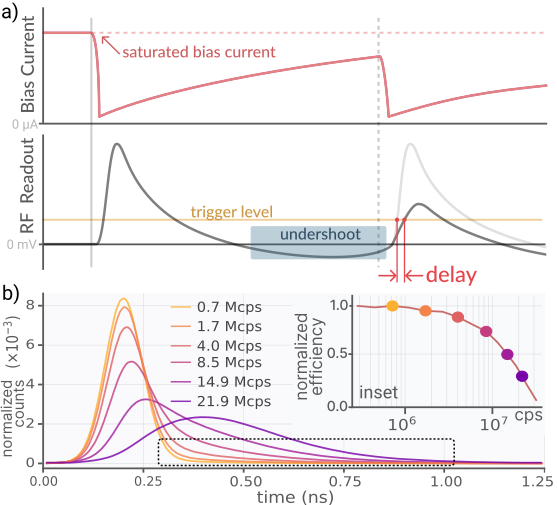
\includegraphics[width=0.7\textwidth,height=\textheight]{./chapter_03/figs/intro_jitterate_light.svg}
\caption[{Introduction to the time walk effect}]{\textbf{Introduction to the time walk effect} a) Diagram illustrating two major sources of correlated high count rate jitter. First, detections may occur during the reset time of a previous detection. At this time the bias current in the nanowire is below its saturated value so that a photodetection triggers an RF pulse with correspondingly lower amplitude. Second, an RF pulse may arrive in the undershoot region of a previous pulse, where the undershoot is a period of negative voltage induced by the low-frequency cutoff properties of the readout amplifier chain. (b) Measured histograms of detections from short $3~\mathrm{ps}$ mode-locked laser pulses. With lower attenuation and higher count rate, the observed timing uncertainty is greater. Inset shows where respective count rates fall on a maximum count rate (MCR) curve \autocite{Zhang_MCR_2019}. The MCR of an SNSPD is often quoted at the $3~\mathrm{dB}$ point, where the normalized efficiency drops to $-3~\mathrm{dB}$ of its maximum value. The jitter increase due to time walk manifests as a tail in the instrument response functions (inside dashed black box) even at count rates significantly below the 3-dB point where detector efficiency has not started to drop significantly (e.g.~the 1.7 Mcps data)}
\label{fig:jitterate_intro}
\end{figure}
}

The time-walk effect in SNSPDs is typically not reported, as jitter is usually measured at low count rates where the detector has ample time to reset following each detection. But as communication and quantum information applications push into higher count rates, the high count rate induced jitter becomes more relevant. LIDAR, quantum and classical optical communication, and imaging applications may all benefit from the development of new detection systems and methods that keep jitter as low as possible in this regime.

We first consider the features of SNSPD operation and readout that cause an increase in jitter with count rate. Then we present multiple ways of mitigating or avoiding these effects, before reviewing our preferred method that relies on a calibration and correction process.

The jitter increase observed at high rate originates from two groups of system characteristics: (i) the intrinsic reset properties of the nanowire, and (ii) properties of the amplification chain. These influence the system's jitter differently, thus it is helpful to consider them separately. Added jitter from either or both sources can emerge when an SNSPD system is operated at high count rates.

The nanowire reset process determines how the detector becomes single-photon sensitive again after a detection. When an SNSPD fires, the current flow in the nanowire momentarily drops to near zero, then recovers in an inverted exponential fashion (Fig.~\ref{fig:jitterate_intro} a). An incident photon may trigger another detection before the bias current fully returns to its saturated value, producing a pulse with a lower amplitude and slew rate. A fixed threshold comparator will trigger on this lower pulse later in time than a full amplitude pulse. If uncorrected for, this time walk manifests as an increase in jitter at high count rates.

The choice of readout amplifiers may also contribute to added high count rate jitter. Pulses may be shifted in voltage and distorted if they arrive when the RF signal has not yet reached a steady zero state following the previous detection. For example, pulses may arrive within an amplifier-induced undershoot region following previous pulses. This phenomenon is illustrated in Fig.~\ref{fig:jitterate_intro} a as the area below 0~mV. The duration of ringing or undershoot effects varies widely depending on the design of the readout circuit. If they last longer than the reset time of the nanowire bias current, the calibration technique may correct for the potentially complex interactions between pulse waveforms that overlap in time.

\hypertarget{jitter-mitigation-methods-at-high-count-rates}{%
\subsection{Jitter Mitigation Methods at High Count Rates}\label{jitter-mitigation-methods-at-high-count-rates}}

There are various methods for correcting for increased jitter at high count rates. These include (i) the use of extra hardware that cancels out some distortions, or (ii) simple software-based data filtering that ignores distorted time-tags. We review these techniques before covering the calibration and correction approach.

Variations in pulse height are a primary component of the distortions that appear at high rates. Such variations in other systems are commonly corrected with a constant fraction discriminator (CFD) that allows for triggering at a fixed percentage of pulse height rather than at a fixed voltage. Adding a CFD to an existing setup is straightforward for a single channel, however it does require additional hardware such as multiple high-speed discriminators and a D-type flip-flop~\autocite{Becker2005}, which significantly increases the circuit complexity and power budget of a multi-channel system. In addition, CFDs are not expected to optimally correct for distortions of the pulse rising edge which may arise from the overlap of one pulse with a signal reflection or undershoot features on the falling edge of a previous pulse. Multi-channel time-to-digital converters (TDCs) used to read out large SNSPD arrays typically only include fixed-threshold comparators~\autocite{Wollman2019}.

In a simple software-based jitter mitigation method, each time-tagged event may be accepted or rejected based on how soon it arrives after the previous pulse. Those that arrive within some pre-determined dead time are assumed to be corrupted by pulse distortions. These are rejected, and the rest are accepted. This method can lower system jitter and maintain high data rates, especially in the cases where only a few percent of pulses are filtered out. However, it can severely limit count rate near the $3~\mathrm{dB}$ point where the majority of counts are rejected (see the supplementary material).

Our correction method preserves original count rate and works with timing measurements from a fixed-threshold free-running TDC -- the type that is often used for SNSPD readout. Pulse pileup correction techniques have been demonstrated with systems that fully digitize detector pulse waveforms~\autocite{Behbahani2019,scoullar_evans_2009,Haselman2010}. But capturing the fast rising edges of SNSPD pulses in this way would require very high sample rates and subsequently, impractically large data streams. In contrast, our method assumes one timing measurement is acquired from triggering on the rising edge of each SNSPD pulse.

We calculate the time between a given \emph{current} SNSPD detection event and a preceding event. This inter-arrival time is used to determine a timing correction for the current event using a lookup table. A calibration routine described next is needed to build this lookup table. Applying these corrections during real-time processing removes deterministic delays correlated with the time between time-tags, leaving only stochastic jitter.

\hypertarget{method-and-results}{%
\section{Method and Results}\label{method-and-results}}

\hypertarget{experimental-setup}{%
\subsection{Experimental setup}\label{experimental-setup}}

The measurements used for calibration and correction were acquired with a high rate mode locked laser (\emph{Pritel}). The minimum repetition rate of this laser was too high to produce a calibration dataset for the Tungsten Silicide detector at highest count rate, given the constraints addressed in the main text. Therefore, the laser was set at a repetition rate of 10.75 GHz and modulated down to 537.5 MHz using two lithium niobate intensity modulators in series. Residual peaks from suppressed mode-locked laser pulses are not observed above the noise floor in the collected data, so their effect was not further considered. Clock jitter is minimized in post-processing with the help of a software-based Phase Locked Loop.

\hypertarget{fig:jitterate_exp_setup}{%
\begin{figure}
\centering
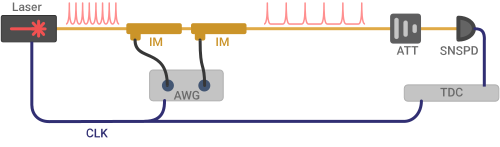
\includegraphics[width=0.9\textwidth,height=\textheight]{./chapter_03/figs/supplemental_expirement_light.svg}
\caption[{Time walk experiment setup}]{\textbf{Experimental Setup} CLK: clock synchronization signal; AWG: Arbitrary Waveform Generator (\emph{Keysight}); IM: Intensity Modulator (\emph{IXBlue}); TDC: Time to Digital Converter (\emph{Swabian Instruments}). The extinction ratio of both modulators exceeds 30 dB.}
\label{fig:jitterate_exp_setup}
\end{figure}
}

\hypertarget{detector-and-trigger-level}{%
\subsection{Detector and trigger level}\label{detector-and-trigger-level}}

We study the pulse distortions observed in a fiber coupled single-pixel tungsten silicide (WSi) SNSPD with 380~$\mathrm{\upmu m^2}$ active area and 160~nm nanowire width. The detector is biased at 9.3~$\mathrm{\upmu A}$, roughly 90\% of the switching current. The readout is handled by a cryogenic DC-coupled amplifier, mounted on the 40~K-stage of the cryostat, which has 43~dB of gain and a 3~dB bandwidth of 700 MHz, followed by a 1~GHz amplifier with 20~dB of gain (\emph{MiniCircuits ZFL-1000LN+}). The system reaches a $3~\mathrm{dB}$ maximum count rate (MCR) of $15.6~\mathrm{MHz}$. The time constant of supercurrent recovery $\tau_{bias} \approx 40~\mathrm{ns}$ is significantly longer than the decay time constant of the RF pulse $\tau_{RF} \approx 5~\mathrm{ns}$, owing to our use of a low-frequency cut-on of $\approx 80$~MHz (-3~dB point from the peak gain) in the DC-coupled amplifiers. For this detector, the calibration process primarily corrects for the lower bias current effects, rather than for any overlapping between RF pulse waveforms (see \textcolor{orange}{supplementary material}). Other detector types and readout systems may operate in a different regime.

The jitter increase with count rate is highly dependent on trigger level. High rate distortions affect the timing measurements less if the threshold voltage is set just above the noise floor.
But triggering on the pulse higher, where it achieves maximum slope, minimizes jitter at low-to-medium count rates. This level varies from 20\% to 50\% of pulse height depending on the detector. We found the minimum low-rate jitter at a trigger level of 50~mV, about 40\% of the pulse height. All further calibration and analysis is performed by triggering at this level in order to optimize jitter across all count rates.

\hypertarget{mode-locked-laser-calibration}{%
\subsection{Mode locked laser calibration}\label{mode-locked-laser-calibration}}

To perform our calibration, we illuminated the SNSPD with an attenuated 537.5~MHz mode locked laser with a mean photon number per pulse between $5\mathrm{e}{-4}$ and $0.016$. The 1.86~ns period of the pulse sequence is large enough that almost all SNSPD detections can be unambiguously matched with a preceding laser pulse -- the period of the pulse train used must be greater than the worst detector jitter for this to succeed. The uncorrected jitter for the WSi detector varies from 50~ps FWHM at low count rates, to about 350~ps at high rates.

\hypertarget{fig:jitterate_explain}{%
\begin{figure}
\centering
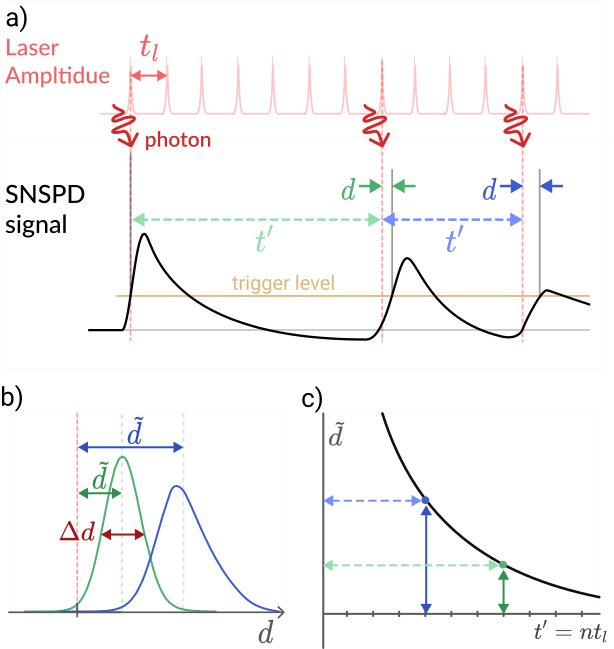
\includegraphics[width=0.7\textwidth,height=\textheight]{./chapter_03/figs/jitterate_explain_light.svg}
\caption[{Calibration method for extracing t' vs delay}]{\textbf{Calibration Method} a) A qualitative diagram illustrating how inter-pulse timing measurements $t'$ and $d$ are extracted. A small fraction of laser pulses contain a photon due to the low mean photon number per pulse of the attenuated laser. Pairs of subsequent photon arrivals are separated by a time denoted by $t' = n t_l$. b) Possible distributions of delay $d$ measurements for two different $t'$. The median of these defines the extracted delay parameters $\tilde{d}$ which form the y-axis in the calibration curve illustrated in (c). The $\tilde{d}$ vs $t^\prime$ curve in (c) approaches zero for $t^\prime$ approaching infinity. Blue and green arrows with matching color and style denote the same measure in (a), (b), and (c).}
\label{fig:jitterate_explain}
\end{figure}
}

We collect sorted time-tags and first consider adjacent pairs of SNSPD events as illustrated in Fig.~\ref{fig:jitterate_explain} a. The time between the two photons that produced these event pairs is defined as $t^\prime$, which is an integer number of laser periods ($t^\prime = n t_{l}$). Second, we derive the delay between the second event and its corresponding laser pulse, defined as $d$. For each laser period spacing $t^\prime$, we make a histogram of the second event delays and find the median ($\tilde{d}$) and the FWHM ($\Delta {d}$) of this distribution. For shorter separations $t^\prime$, the distribution is expected to have larger delays and FWHM (Fig.~\ref{fig:jitterate_explain} b) due to the smaller pulse height of the second event. Finally, we use the median delay as a function of laser spacing (Fig.~\ref{fig:jitterate_explain} c) to form a curve $\tilde{d}$-vs-$t^\prime$ for the added time-walk versus inter-arrival time.

\hypertarget{fig:jitterate_results_1}{%
\begin{figure}
\centering
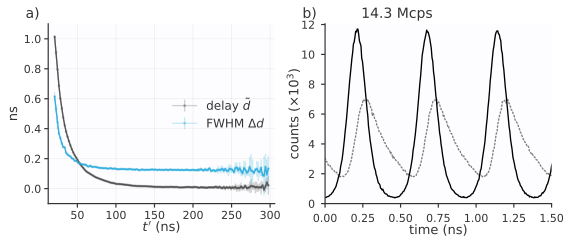
\includegraphics[width=0.9\textwidth,height=\textheight]{./chapter_03/figs/jitterate_data_ab_light.svg}
\caption[{t-prime curve and correction effect}]{\textbf{t-prime curve and correction effect} (a) Delay and intrinsic jitter curves extracted from the 537.5 MHz pulsed light dataset. (b) Histogram of corrected (black) and uncorrected (dashed grey) time tags from a 2.15 GHz pulse train, corrected using a calibration curve developed with the 537.5 MHz dataset. The improvement affirms that the light modulation used for an application need not match the repetition rate of the calibration laser.}
\label{fig:jitterate_results_1}
\end{figure}
}

Fig.~\ref{fig:jitterate_results_1} a shows the $\tilde{d}$-vs-$t^\prime$ and $\Delta d$-vs-$t^\prime$ curves collected from our measurements of the WSi detector. The $\tilde{d}$-vs-$t^\prime$ curve is the main result of the calibration process and is used as a lookup table in the correction method. $\Delta d$ is a measure of the more intrinsic jitter that the correction method cannot cancel out. While it is larger for small $t^\prime$ due to triggers on lower amplitude pulses, it notably stays at a nearly minimized value down to around $t^\prime =$ 50~ns. $\tilde{d}$ grows more dramatically with decreasing $t^\prime$, especially in the range from 50~ to 100~ns. For count rates that don't exhibit many inter-pulse arrival times smaller than 50~ns, a method for removing the time-walk effect's contribution to jitter should bring entire system jitter back down to near the intrinsic limit implied by the $\Delta d$ curve.

The correction method we implement involves subtracting off the distortion-induced delays a time-tag is expected to have based on the inter-pulse-time that precedes it. For each time tag $t_n$ in a set, the inter-pulse time is $t_n - t_{n-1} = \Delta t$, where $t_{n-1}$ is the previous tag on the same channel. Using $\Delta t$ as an index, a corresponding delay correction $\hat{d}$ is found by interpolating the $\tilde{d}$-vs-$t^\prime$ curve from the calibration. Given the density of points in the $\tilde{d}$-vs-$t^\prime$ acquired here, a linear interpolation is sufficient. The correction may benefit from higher order interpolation if the $\tilde{d}$-vs-$t^\prime$ curve is more sparse. This would be the case for calibrations built from a slower repetition rate pulsed light source. An assumption underlying the correction is that the interpolated value $\hat{d}$ is a good estimator of the true delay added to the current time-tag due to high count rate pulse distortions.

With the interpolation operation expressed as a function $D$, the correction is written as $\overline{t}_n = t_n - D(\Delta t)$, where $\overline{t}_n$ is the corrected version of tag $t_n$. Whether $t_{n-1}$ is itself corrected or uncorrected has negligible influence on the $t_n$ correction, as we assume $d << \Delta t$. The data correction shown here was applied in post-processing. But since $D$ depends only on the current time tag and information available from earlier, the correction can be applied in real-time in an FPGA or computer used for time tagging.

\hypertarget{fig:jitterate_results_2}{%
\begin{figure}
\centering
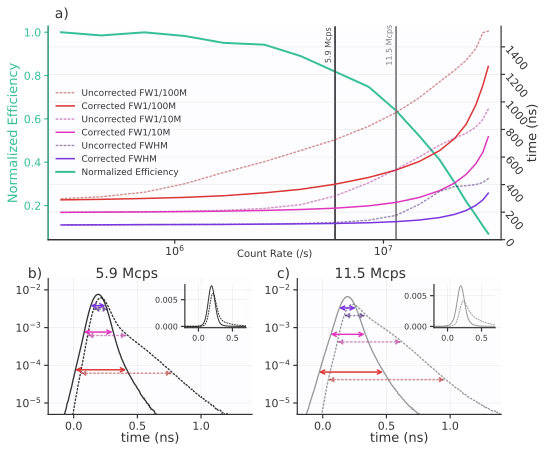
\includegraphics[width=0.9\textwidth,height=\textheight]{./chapter_03/figs/jitterate_data_c_light.svg}
\caption[{Jitters metrics across incident powers}]{\textbf{Jitters metrics across incident powers} (a) Effect of the correction on measurements of system jitter over a range of rates approaching the maximum count rate. (b) Corrected (solid) and uncorrected (dashed) instrument response functions with color-matched arrows showing the location of the width-statistics plotted above in (a). The black vertical line in (a) is drawn at the count rate of this plot. Inset shows linear scaling. (c) Corrected (solid) and uncorrected (dashed) histogram analogous to (b), but at a higher count rate indicated by the grey line in (a).}
\label{fig:jitterate_results_2}
\end{figure}
}

The correction we perform using the $\tilde{d}$-vs-$t^\prime$ curve in Fig.~\ref{fig:jitterate_results_1} a is applicable to a wide range of count rates and arbitrary modulation patterns; there is no requirement that applications match the repetition rate of the calibration laser. Fig.~\ref{fig:jitterate_results_1} b shows that the correction method, derived from the 537.5 MHz calibration data, significantly reduces jitter when applied to detections from a 2.15~GHz pulse train. A similar jitter reduction can be demonstrated for repetition rates below 537.5~MHz.

To study the effectiveness of our correction method at different count rates, we apply it to data collected at different mean photon numbers per pulse, with the same 537.5 MHz pulse train. As shown in Fig.~\ref{fig:jitterate_results_2} c, the correction improves the FWHM at rates approaching the 3~dB point, and improves FW10\%M and FW1\%M (full width at ten percent/one percent maximum) dramatically, even at count rates significantly below the 3 dB point, where detector efficiency is nearly maximized. This reduction is evident in Fig.~\ref{fig:jitterate_results_2} c, where the correction works to remove a time-walk induced tail in the instrument response function. The ratio of corrected FW1\%M over uncorrected FW1\%M reaches a minimum of 0.55 at a count rate of 11.5 MCounts/s. Therefore if an application sets its repetition rate or bin size based on the FW1\%M metric, the repetition rate can be increased and the bin size decreased by up to 45\% without any increase in event misattribution errors. These improvements are notable for applications including biomedical imaging~\autocite{Sutin16,Bruschini2019}, quantum communication~\autocite{Hadfield2009} and laser ranging~\autocite{McCarthy13} that have stringent timing requirements over a large dynamic range.

\hypertarget{higher-order-correction-the-peacoq-detector}{%
\section{Higher order correction \& the PEACOQ detector}\label{higher-order-correction-the-peacoq-detector}}

The Performance Enhanced Array for Counting Optical Quanta (PEACOQ) is a new fiber-coupled SNSPD design that achieves high count rate by spreading the photon flux across a parallel array of short niobium nitride nanowires. Each wire may acheive count rates as high as 50 MCounts/s, so the 32-wire array as a whole can handle photon rates in excess of 1 GCounts/s. The PEACOQ is described in detail in Reference \autocite{Craiciu23}.

From early tests of the PEACOQ, it became evident that jitter increased dramatically at high single wire count rates. One of the overaching goals the the PEACOQ project was to demonstrate near-100~ps jitter at 1 GCount/s. Therefore, we investigated the possibility of applying time walk correction techniques to this detector. This began with collecting a calibration dataset like that discussed in section \ref{mode-locked-laser-calibration}.

A 1-GHz repetition rate 1550 nm mode locked laser was used (Pritel UOC) for calibration. The 1~GHz repetition rate was chosen so that uncorrected jitter even at the highest count rates (approaching 400 ps at the FW1\%M), was smaller than the laser period. Then, each time tag may be matched to the timing of the original optical pulse. A dataset with a count rate of 20 MCounts/s was used for calibration. At this rate, there is a good balance of statistics available for $t'$ ranging between 5 and 150 ns.

The calibration process for the PEACOQ showed that high-rate pulse distortions are primarily due to amplifier effects and the overlap of RF pulses with the overshoot or ringing effects of previous RF pulses. This is because the nanowire design and fabrication of the PEACOQ seeks to minimize the intrinsic reset time of the nanowire. The time it takes for bias current to re-saturate in the device is generally faster than the time for all amplifier effects to disappear following a previous RF pulse. Fig.~\ref{fig:order_1st} b is the delay vs.~$t’$ curve derived from the calibration process. Unlike the in Fig. \ref{fig:jitterate_results_1}, the delay vs.~$t’$ curve for the PEACOQ shows features that are closely related to the falling edge of the RF pulse (Fig.~\ref{fig:order_1st} a). In particular, the calibration curve shows a peak near 25 ns that aligns with an undershoot in the RF waveform caused by a reflection off a cryogenic amplifier. Future implementations of the PEACOQ will optimize the amplification chain to minimize RF reflections. Though even with such optimizations, it is likely that time-walk correction will improve high rate jitter.

\hypertarget{fig:order_1st}{%
\begin{figure}
\centering
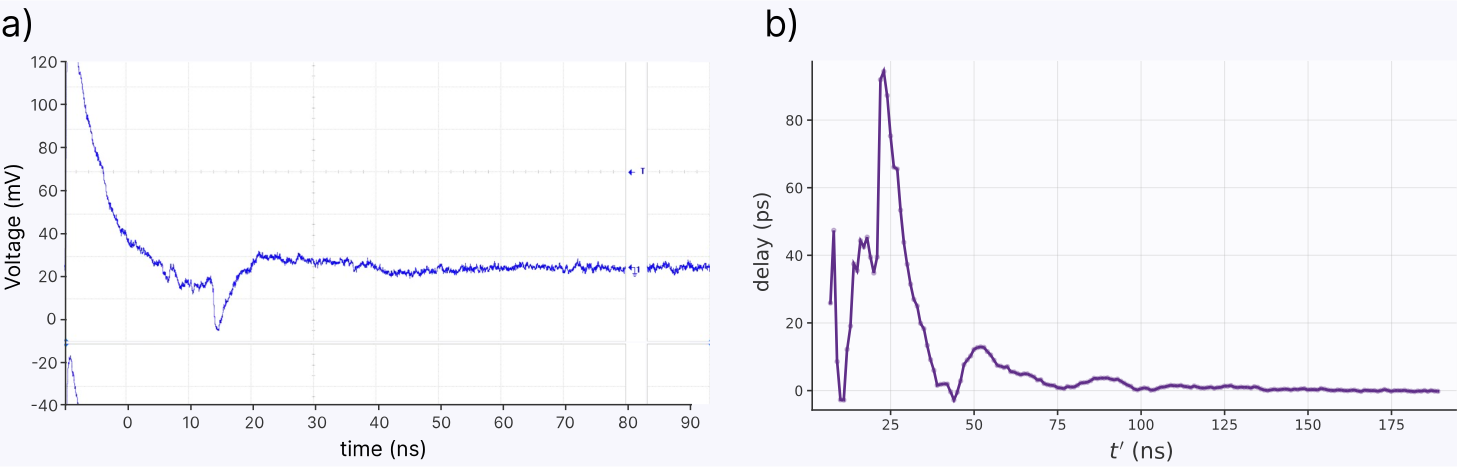
\includegraphics[width=1\textwidth,height=\textheight]{./chapter_03/figs/SOM_Figure_order_1st_v2_light.svg}
\caption[{PEACOQ RF pulse and calibration curve}]{\textbf{PEACOQ RF pulse and calibration curve} a) The RF pulse of one of the PEACOQ nanowires. The effect of an impedance mismatch reflection is visible at 25~ns. b) The delay vs $t'$ curve for wire 1 of the PEACOQ. The peak at 25~ns lines up in time with the RF reflection visible in (a), and works to correct for the time-walk delays it causes.}
\label{fig:order_1st}
\end{figure}
}

As before with the meandered SNSPD, there is no requirement that the calibration only be used in an application that's based on the same repetition rate of 1 Ghz. As interpolation between points on the delay vs.~$t'$ vslookup curve is possible, delay corrections for arbitrary $t'$ measurements may be found.

\hypertarget{second-order-calibration}{%
\subsubsection{Second Order Calibration}\label{second-order-calibration}}

The 2nd order time-walk correction is a new technique that builds on the methods previously introduced in this chapter. The intrinsic reset time of the PEACOQ nanowires is considerably shorter than the time it takes an RF pulse to return to a steady zero voltage. So multiple pulses can arrive in the time it takes one RF pulse to fully decay as seen by the timing electronics. Therefore, a given RF pulse can be level shifted not only by the presence of a previous pulse a few nanoseconds earlier, but even by the presence of two previous pulses. The calibration and correction process was extended to correct a given pulse timing measurement based on two inter-pulse time measurements $t'$ and $t''$ as shown in Fig.~\ref{fig:order_2nd} a. The calibration process uses the same mode-locked laser derived pulse train as the 1st order calibration. For each $t'$ there is a full range of possible $t''$ times and vice versa, so the result of calibration becomes a 2D grid of delay corrections indexed by $t'$ and $t''$. $t'$ is always less than $t''$ for the parameterization chosen, where both are measured from the latest or `current' time tag (Fig.~\ref{fig:order_2nd} a). Therefore, the space of valid measurements is triangular as shown in Fig.~\ref{fig:order_2nd} b.

\hypertarget{fig:order_2nd}{%
\begin{figure}
\centering
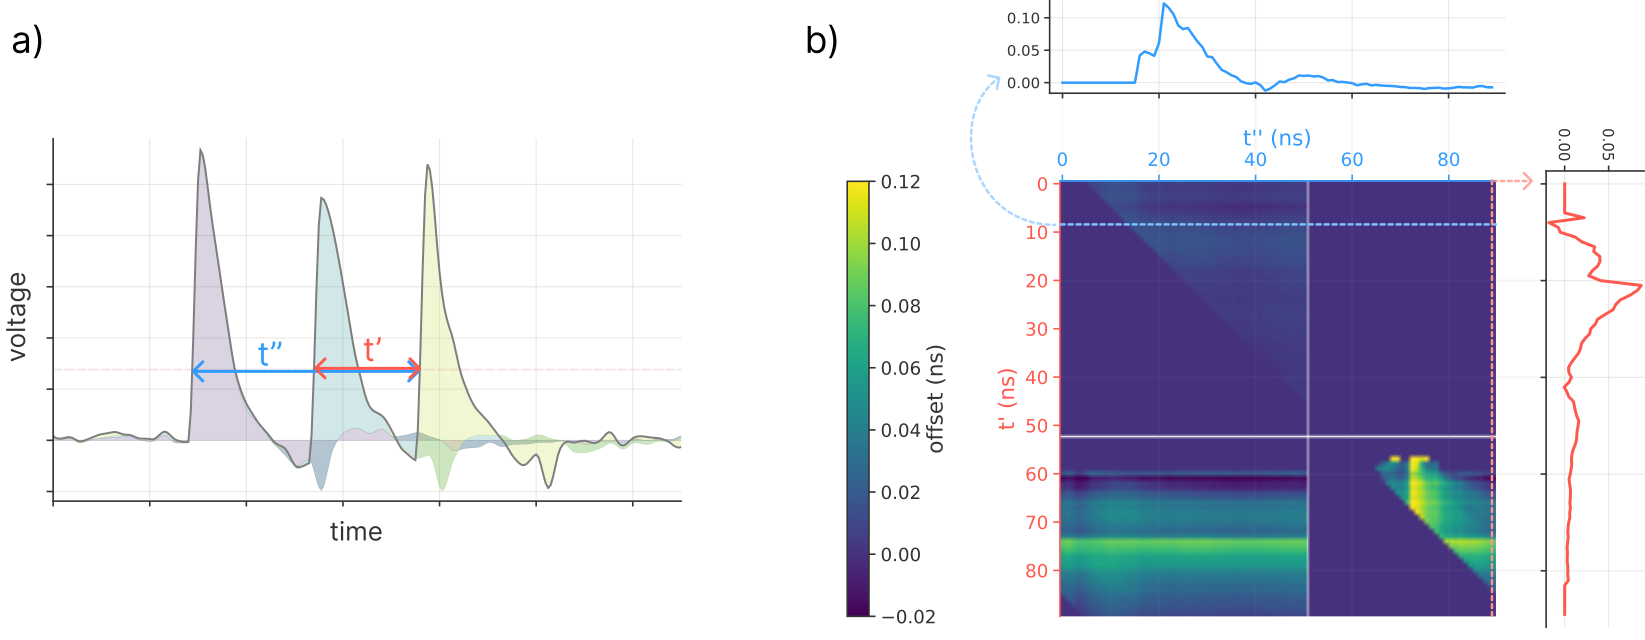
\includegraphics[width=1\textwidth,height=\textheight]{./chapter_03/figs/SOM_Figure_order_2nd_v1_light.svg}
\caption[{PEACOQ 2D calibration parameterization \& results}]{\textbf{PEACOQ 2D calibration parameterization \& results} a) A diagram showing how RF pulse waveforms can interfere additively, and how $t'$ and $t''$ are parameterized. For illustrative purposes only. b) The result of 2nd order calibration, a grid of delay measurements indexed by $t'$ and $t''$. The blue/red slices and corresponding graphs show how the the effect of varying $t''$ for a given $t'$ is similar to varying $t'$ for a given $t''$.}
\label{fig:order_2nd}
\end{figure}
}

Predominant features of the 2d calibration grid seem to be orthogonal and aligned to the axes. This is a result of the parametrization chosen for $t'$ and $t''$. Features of the calibration that arise due to additive mixing of overlapped RF pulse waveforms which manifest as orthogonal structures in the 2d-calibration grid.

In the limit of large $t''$, a slice of the calibration grid bears close resemblance to the $t'$ vs delay curve used for 1D calibration and correction (Fig.~\ref{fig:order_1st} b). Like in the 1D correction method, a delay correction can be found during real-time acquisition and processing by interpolating on a lookup table. Only now, the lookup table has an extra dependent variable $t''$, and the interpolation is two dimensional.

Proper handling of inter-pulse arrival measurements that fall outside the 2D grid is necessary for good correction performance. When both $t'$ and $t''$ fall outside the 2D grid, no correction is applied. When $t''$ falls outside the grid but $t'$ does not, a 1st order correction is applied to determine what delay must be subtracted to the current tag to correct its distortion. When both $t''$ and $t'$ fall within the 2d grid, a full 2d spline interpolation on the grid in Fig.~\ref{fig:order_2nd} b is applied to find the necessary delay correction.

Like the 1st-order correction, the 2nd-order method makes the assumption that the delays to be corrected are small relative to the inter-pulse times $t’$ and $t’’$.

The codebase supporting our findings with the 1st and 2nd order correction is
available at \href{https://github.com/sansseriff/SNSPD-time-walk-and-jitter-correction}{SNSPD-time-walk-and-jitter-correction}.

{}

\hypertarget{performance-regime-of-the-tungsten-silicide-detector}{%
\subsection{Performance Regime of the Tungsten Silicide detector}\label{performance-regime-of-the-tungsten-silicide-detector}}

When our calibration and correction method is applied to the Tungsten Silicide SNSPD, the walk-cancellation method primarily corrects for pulse height variations. These variations are caused by varying levels of bias current in the device at the time of photo-detection. An oscilloscope trace shows an exponentially decaying increase in SNSPD pulse height following a previous detection. This exponential recovery shape reinforces evidence that this detector operates in this `bias current recovery' regime, rather than the regime where amplifier reset dynamics dominate.

\hypertarget{fig:rise_exp}{%
\begin{figure}
\centering
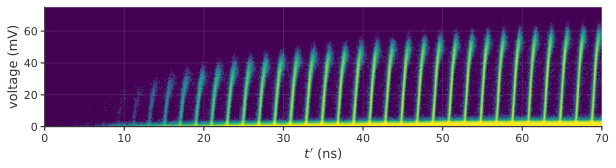
\includegraphics[width=1\textwidth,height=\textheight]{./chapter_03/figs/rise_exp_light.svg}
\caption[{WSi pulse exponential pulse recovery}]{\textbf{WSi detector pulse recovery} Sweep of trigger levels for pulse rising edges after a previous pulse (not shown). This is similar to a scope trace in overlay false color mode. The detector is illuminated by a 537.5 MHz pulse train.}
\label{fig:rise_exp}
\end{figure}
}

\hypertarget{software-dead-time-for-high-count-rate-jitter-suppression}{%
\subsection{Software dead time for high count rate jitter suppression}\label{software-dead-time-for-high-count-rate-jitter-suppression}}

In certain cases a software-based dead time is an effective way of reducing jitter at high count rates. SNSPD pulses that arrive soon after a previous pulse are ignored because their timing is assumed to be corrupted due to pulse distortions (Fig. \ref{fig:dead_time}a). With a long software-based dead time, data is filtered to keep only events for which the SNSPD was in a fully reset state prior to detection. This results in low jitter measurements even at high rate as shown in Fig. \ref{fig:dead_time}d where the dashed and solid (red, orange) lines are response functions of unfiltered and filtered data respectively. However, the use of software-based dead times can severely limit usable count rate. This paradoxically contrasts with the main intended goal, which is to operate an SNSPD at the highest possible count rates. As shown in the Fig. 3b, adding a 100 ns software dead time to our WSi single pixel SNSPD limits its usable maximum count rate to about 4 MHz, while the raw count rate exceeds 10 MHz. Furthermore, the usable count rate drops to zero for higher incident photon rates, as the dead time starts to reject most events. This behavior can be unexpected and problematic for any applications that occasionally over-saturate the detector.

\hypertarget{fig:dead_time}{%
\begin{figure}
\centering
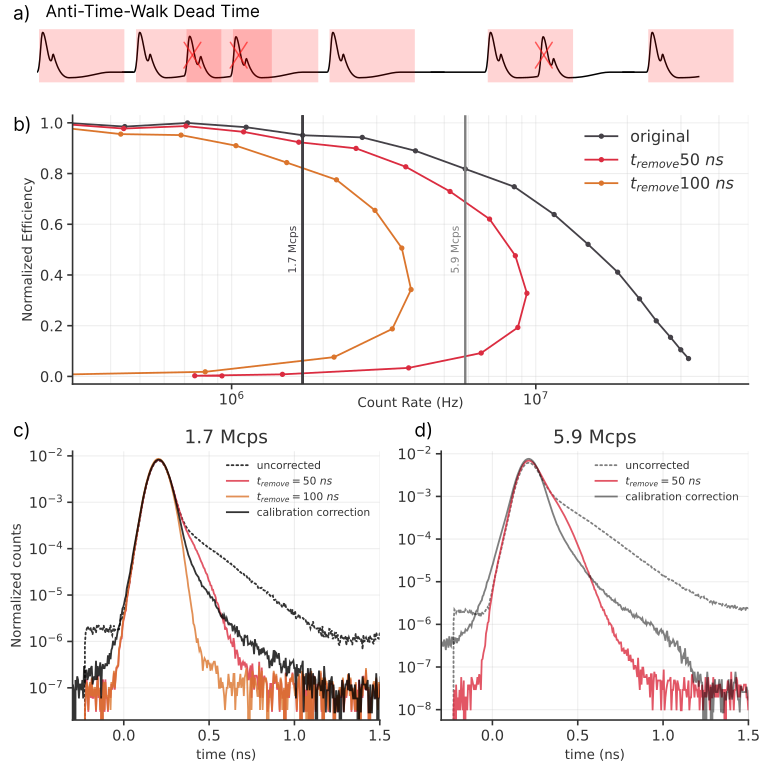
\includegraphics[width=0.8\textwidth,height=\textheight]{./chapter_03/figs/cut_count_rate_v2_light.svg}
\caption[{Removing time walk with dead time}]{\textbf{Removing time walk with dead time} a) Illustration of the RF signal out of an SNSPD with red highlighted regions signifying a software-based dead time that rejects some events. b) Count rate vs normalized efficiency, similar to the curve in green in Fig.~\ref{fig:jitterate_results_2}. (c) \& (d) Response functions for timetaggs at two count rates denoted by the vertical lines in (b), similar to Fig.~\ref{fig:jitterate_results_2} (b) and (c). The dark grey solid lines show response functions from the calibration and correction method which does not limit count rate. The 100 ns dead time filtered data does not reach the 5.9 Mcps of figure (d) and is therefore not shown in (d).}
\label{fig:dead_time}
\end{figure}
}

\hypertarget{conclusion-outlook}{%
\section{Conclusion \& Outlook}\label{conclusion-outlook}}

The original research paper on time walk analysis \autocite{Mueller2023} included comments on the potential for time walk correction in situations where the reset reset time of the nanowire is considerably shorter than the reset dynamics of the amplifier chain:

\begin{quote}
To optimally correct for this, higher-order correction techniques are needed based on higher-dimensional lookup tables. There is an avenue for exploring such methods for unique use-cases. \autocite{Mueller2023}
\end{quote}

This potential for higher order correction methods turned out to be fruitful, which is why the prior section about \href{section_05_peacoq_2nd_order.md\#second-order-calibration}{higher corder correction} adapted from the PEACOQ paper \autocite{Craiciu23} is included. The original paper went on to claim that there are avenues for exploring time walk correction for pulses measured at multiple voltage levels, or even fully digitized pulses captured with high speed ADCs and FPGAs. These more rigorous readout techniques may be needed to deconvolve photon timing and Photon Number Resolution (PNR) effects from the same nanowire at high count rates~\autocite{Hao2021}. While drafting this thesis, methods for simultaneous time walk correction and PNR correction have not been demonstrated in the literature. However, I believe there is imminent potential to extend the gaussian mixture model methods introduced in the next section for these purposes.

There are other types of extensions and modifications to the presented time walk correction method that may prove to be useful. However, the single-$\Delta t$ measurement approach primarily detailed in this chapter is broadly applicable and straightforward to implement. For insight into developing a streamlined calibration process and in-situ time walk correction as part of larger quantum communication experiments, see the time walk correction section in the chapter 4 \textcolor{orange}{include link}.

As applications like LIDAR and quantum communication demand ever higher data rates, multiple techniques for increasing photon and data throughput of SNSPD systems are being explored. Arrays or multi-channel SNSPD systems will play a role in satisfying that demand. However, compared to multiple lower count rate SNSPDs operating in parallel, a single detector operating at high rate has certain advantages. First, it makes more efficient use of the extensive bandwidth of the RF readout channel. Second, the single detector with single readout line puts less thermal load on the cooling system than multiple detectors with multiple readout lines. Therefore, paths toward operating individual SNSPDs at the limits of their count rate performance should be explored before extending to multi-pixel systems. This work is a step towards unlocking all available performance and timing precision of SNSPDs operated at high count rates.

\hypertarget{data-recovery-and-pulse-position-modulation-with-a-photon-number-resolving-snspd}{%
\chapter{Data Recovery and Pulse Position Modulation with a Photon Number Resolving SNSPD}\label{data-recovery-and-pulse-position-modulation-with-a-photon-number-resolving-snspd}}

A version of this chapter will be submitted the the journal optics express. A preprint is released as \textcolor{orange}{arxiv citation here}

\hypertarget{abstract-2}{%
\section{Abstract}\label{abstract-2}}

Superconducting Nanowire Single Photon Detectors are a type of time-correlated photon detector with low jitter performance especially in the mid-infrared. They are useful for classical communication over high loss channels --such as across deep space-- and for quantum communication for which signals are restricted to the few-photon level. For classical communication, high photon information efficiency communication may be achieved with Pulse Position Modulation (PPM) whereby data is encoded in the arrival time of an optical pulse with respect to a clock. In the process of demonstrating PPM on a 20~Ghz clock, we study the effects of Photon Number Resolution (PNR) in new low-jitter types of SNSPDs. These PNR effects complicate fixed-threshold triggering of RF pulses from the SNSPD, and corrupt arrival time measurements if not properly managed. We demonstrate methods for simultaneous arrival time and photon number measurement which enables high clock rate PPM for space applications as well as high rate quantum communication and computing applications that benefit from photon number resolution.

\hypertarget{introduction-3}{%
\section{Introduction}\label{introduction-3}}

Deep space optical communication has been a growing field of study in recent years, as space agencies look for ways to increase data rates to and from deep space missions. A key challenge in the development of this technology is closing the communication link over extremely large distances and high loss. This must be done given a restricted power budget available on the spacecraft, and therefore requires the use of photon efficient communication protocols that optimize the number of bits sent per unit of energy.

In this article, we demonstrate high rate Pulse Position Modulation (PPM) applicable to future deep space communication. This starts with a transmitter that sends an optical pulse in one of $2^M$ possible time slots measured with respect to a clock. At a receiver, the arrival time of this pulse is measured to recover $M$ bits of encoded data. Each successive set of $2^M$ time slots following by a dead time constitute a PPM frame.

The Deep Space Optical Communicaiton (DSOC) project managed by the Jet Propulsion Laboratory (JPL) aims to demonstrate optical communication using PPM with the Psyche spacecraft from distances of 0.06 to 2.7 Au \autocite{Srinivasan2023GroundReceiver}.

For larger M, more data may be sent with a single optical pulse, thereby allowing a power limited spacecraft to send more data over a high loss optical channel back to earth. This is quantified through the photon information efficiency $c_p = C/E$ where $C$ is the link capacity and $E$ is the photon cost per optical pulse

The DSOC project uses M at least as high as 5, meaning 5 bits of data are send using 32 time slots per frame. M values as high as 19 have been demonstrated in the lab~\autocite{essiambre2023record}, but the number of time bins needed per frame scales exponentially with the number of bits transmitted per pulse. Therefore, for a given fixed clock rate and time bin duration, the PPM data rate decreases dramatically for higher M values.

We demonstrate a high clock rate PPM protocol in the lab based on modulating a mode-locked laser and receiving pulses with a low jitter superconducting nanowire single photon detector (SNSPD) (Fig.~\ref{fig:intro} (a)).We focus on demonstrating moderately large PIE, while also increasing the clock rate of the sytem by an order of magnitude relative to the DSOC platform (2~GHz). By operating at both higher clock rate and PIE than DSOC, this system exemplifies how future iterations of DSOC may send data more quickly but also over greater distances with the same power budget.

The rate increase is possible due to recent advancements in Niobium Nitride SNSPDs~\autocite{Colangelo2023}. These achieve low jitter performance by incorporating impedance matching tapers for efficient RF coupling, resulting in higher slew rate pulses, and by enabling RF pulse readout from both ends of the nanowire. The dual-ended readout allows for the cancellation of jitter caused by the variable location of photon arrival along the meander when the differential signals are recombined with a balun. These detectors achieve jitter as low as 50 ps at the FW(1/100)M level, making them suitable for the demonstration of PPM with 50 ps slot widths and a 20 GHz clock.

\hypertarget{fig:intro}{%
\begin{figure}
\centering
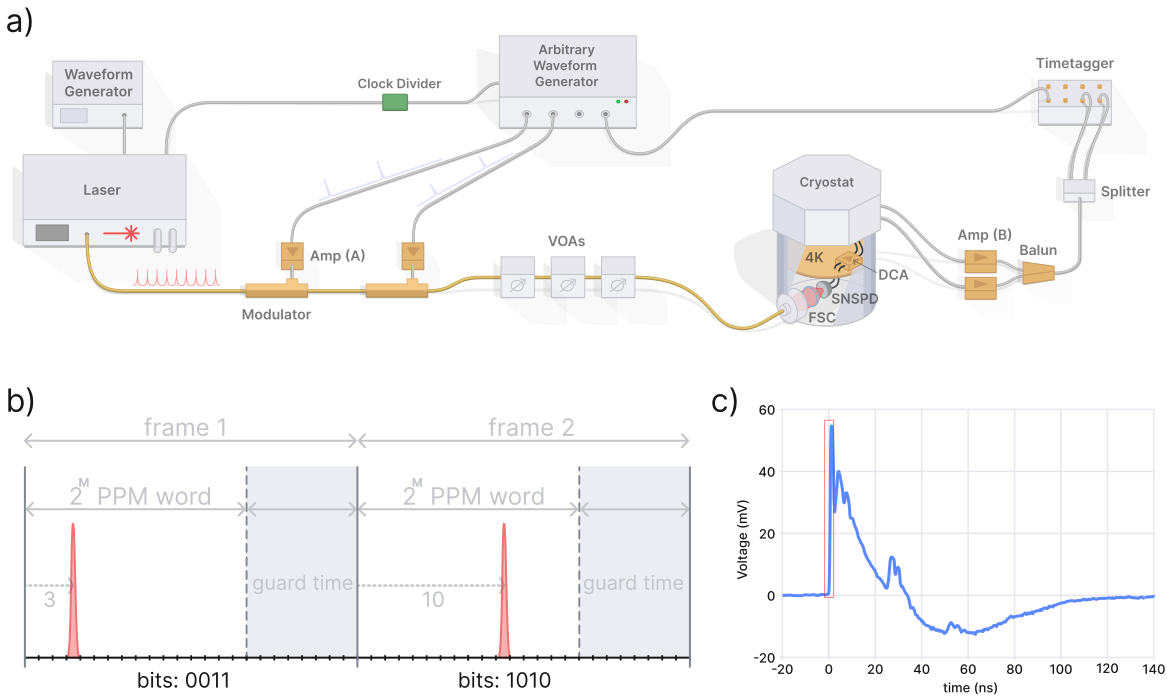
\includegraphics[width=1\textwidth,height=\textheight]{./chapter_04/figs/fig_intro_2_light.svg}
\caption[{PPM modulation and experiment setup}]{\textbf{PPM modulation and experiment setup} a) Diagram of the expiremental setup. WG: wave generator, CD: clock divider board, AWG: Arbitrary Waveform Generator, MLL: Mode Locked Laser (Pritel UAC), IM: Intensity Modulator, BC: Bias Controller, FSC: Free Space Coupling System, DCA: DC Coupled Cryo-amp b) How bits are transmitted in M=16 PPM modulation. An optical pulse is transmitted with a clock-referenced integer delay which encodes 4 bits of data. c) Scope trace of the RF pulse produced by the differential-readout tapered SNSPD. Fig.~\ref{fig:waveform} zooms in on the rising edge outlined in red here}
\label{fig:intro}
\end{figure}
}

However, these detectors exhibit photon number number dependent responses that affect the time-correlated measurements needed for high-rate PPM. This behavior, shown in Fig.~\ref{fig:waveform} is also known as photon number resolution (PNR) -- a property that is desirable in certain applications including quantum communication and quantum computing. The SNSPD generates RF pulses with greater amplitude and slew rate when detecting optical pulses with multiple photons. Photon number effects are especially evident in this lower jitter variety of SNSPD due to the use of impedance matching tapers which more efficiently couple energy out of the nanowire and into the readout circuit. With high resolution time tagging equipment, photon number dependent effects have even been observed in SNSPDs not necessarily designed to exhibit it \autocite{schapeler2023superconducting,sauer2023resolving} like those without tapers \autocite{Cahall2017SlewRatePNR}. Therefore it is increasingly likely that future research involving low-jitter SNSPDs and multiphoton pulsed sources will have to explicitly manage the PNR response for accurate time-correlated measurements -- whether the effect it is desired or not.

For the tapered differential detectors, the PNR response affects timing of fixed threshold timetaggs at any trigger level (Fig.~\ref{fig:waveform}). However, at higher trigger levels the PNR response is less pronounced and the timing measurements are less affected. Therefore, we divide a single SNSPD readout line using an RF splitter and trigger on the RF pulse at a high and low level as shwon by the red lines in Fig.~\ref{fig:waveform}. This allows us to extract the somewhat conjugate information of pulse arrival time and photon number. From these measurements we study the PNR response in detail and present two methods for managing it. We demonstrate how the photon number information may be deconvolved from the arrival time information, and how both de-correlated degrees of freedom can be extracted simultaneously. This enables the original goal of high rate PPM, but also informs how low-jitter photon number resolving SNSPDs can be used in other classical communication and quantum applications.

\hypertarget{fig:waveform}{%
\begin{figure}
\centering
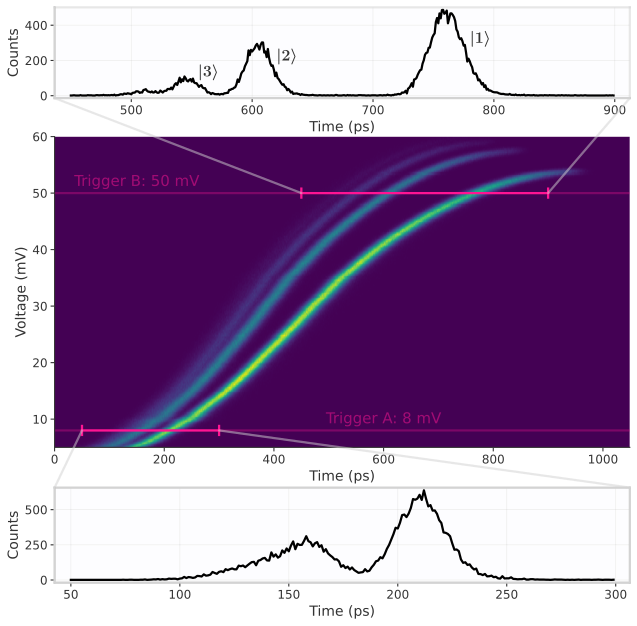
\includegraphics[width=0.8\textwidth,height=\textheight]{./chapter_04/figs/waveform_light.svg}
\caption[{PNR-sensitive Pulse Waveform}]{\textbf{PNR-sensitive Pulse Waveform} The rising edge of the differential SNSPD's RF pulses exhibit variations in height, slew rate, and arrival time due to photon-number dependent dynamics. The slopes of the 1-photon and 2-photon pulses significantly differ, and as the photon number increases, the alterations to the pulse shape become progressively smaller. Trigger levels A (8~mV) and B (50~mV) were used to extract as much information about pulse slope and arrival time as possible}
\label{fig:waveform}
\end{figure}
}

\hypertarget{detector-figure-of-merit}{%
\section{Detector Figure of Merit}\label{detector-figure-of-merit}}

The work here highlights the application of low jitter single-photon detectors for optical communication, which is impactful for deep-space optical communication as well as classical communication in quantum networks. Although single-photon counting is well estanblished for deep-space optical communication~\autocite{Srinivasan2023GroundReceiver} so far it has not been ulitized in quantum networks, mainly due to the use of SFP modules and DWDMs. However, with the eachievement of high data rates recently achieved with photon-counting classical communication, these approaches can now be seriously considered for quantum networks. The main driver is the reduction of optical power in neighbouring DWDM channels, which ultimately lowers the Raman scattered photons into the quantum channel \autocite{EraerdsRaman}
\textcolor{orange}{Calculate reduction in power from state of the art SFP modules}

To access the applicability of different detectors, here we compare some of the recent near infrared detectors.

A useful figure of merit that includes all of the revelant detector metrics for photon timing was introduced by Bronzi and co-authors \autocite{Bronzi2016}

$$FoM_T = \frac{\eta  (1 - P_{ap})\Phi_{-3 \text{dB}}}{J} \sqrt{\frac{A}{D}},$$

where $\eta$ is the single photon detection efficiency, $\Phi_{-3 \text{dB}}$ is the photon flux at which the system detection efficiency drops by 3~dB, $P_{ap}$ is the afterpulsing probability, $J$ is the detector jitter evaluated as the FWHM, $T_d$ is the deadtime, $A$ is the active area and $D$ is the dark count rate. Here we have defined the maximum photon flux as the 3~dB point, for ease of standardization.

In this work:

\begin{itemize}
\tightlist
\item
  Efficiency = 0.84
\item
  Afterpulsing = 0 \%
\item
  Jitter = 15 ps
\item
  Deadtime = 30 ns \textcolor{orange}{measure 3dB flux}
\item
  Area = 330 $\mu m^2$
\item
  Dark count rate = 20~Hz
\end{itemize}

$FoM_T = 7.58 \times 10^{12}$ at 1550 nm.

The deadtime is calculated as the 1/MCR, which is the 3 dB point of the nominal efficiency. This is only a factor of 3.7 less than the state of the art visible Silicon SPADs (peak efficiency at 480~nm) \autocite{Gramuglia2022}

In the future, the performance of the optical communication system could be improved by using, high count rate SNSPD arrays. Recently published high-count rate arrays have figures of merit of \textcolor{orange}{$FoM_T$ for Peacoq and Resta2023 results}. This would result in a proportinal increase in the data rate.
\textcolor{orange}{$FoM_T$ for fastest InGaAs/InP gated detector}
These devices are ideal for fiber-based optical communication. In free-space, the active area is especially important, whithout the use of an adaptive optics system.
\textcolor{orange}{$FoM_T$ for DSOC array}

\hypertarget{development-of-a-modulation-source}{%
\subsection{Development of a modulation source}\label{development-of-a-modulation-source}}

DSOC relies on modulation of a CW seed laser to generate the communication signal on the spacecraft. This signal is then amplified by an Erbium Doped Fiber Amplifier (EDFA) to increase its transmission power to Earth. As the EDFA amplifies the pre-generated pulses and uses most of the power of the spacecraft optical transmission system, power consumption scales with the number of optical pulses.

We produce our PPM signal signal by carving a high rate mode locked laser with lithium niobate modulators. This way, the jitter of the optical pulses themselves are not limited by the modulators or slew slew rate of the RF signal that drives them. We do two PPM demonstrations, with the source mode locked laser operating at 10.75 and 20 GHz. THe 10.75 GHz demonstration uses a M value of 10, thereby making frames with 1024 time slots of 93 ps width each. The 20 GHz demonstration uses M=11, giving 2048 time slots of 50 ps width per frame. Each frame ends with a dead time of approximately 150 ns to allow the SNSPD to fully recover before the next frame.

Several modern free running time taggers support the averaging of multiple input channels to create fewer higher resolution channels. This implies a tradeoff between jitter or timing resolution and number of channels for a given time tagging device. Therefore, it is important to consider readout methods like that presented here that make use of 2 lower-resolution channels in place of a single higher resolution channel, as these two configurations are similarly resource efficient.

\hypertarget{methods}{%
\section{Methods}\label{methods}}

Prior to the PPM demosntration, we collected data with multi-photon optical pulses repeatedly impinging on the detector at the same time with respect to a clock. This way, we study how the PNR effect in isolation is manifest in the timing measurements recorded at the low and high trigger levels. We label the measurements from the low (8~mV) and high (50~mV) trigger levels as $t_A$ and $t_B$ respectively. As shown in Fig.~\ref{fig:waveform}, histograms of these arrival events are multimodal due to the PNR response. We first present a method for recovering a symmetric arrival time response function using the the slope measurement $\Delta t_{BA} = t_B - t_A$.

\hypertarget{slope-based-correction}{%
\subsection{Slope-Based Correction}\label{slope-based-correction}}

\hypertarget{fig:slope_correction}{%
\begin{figure}
\centering
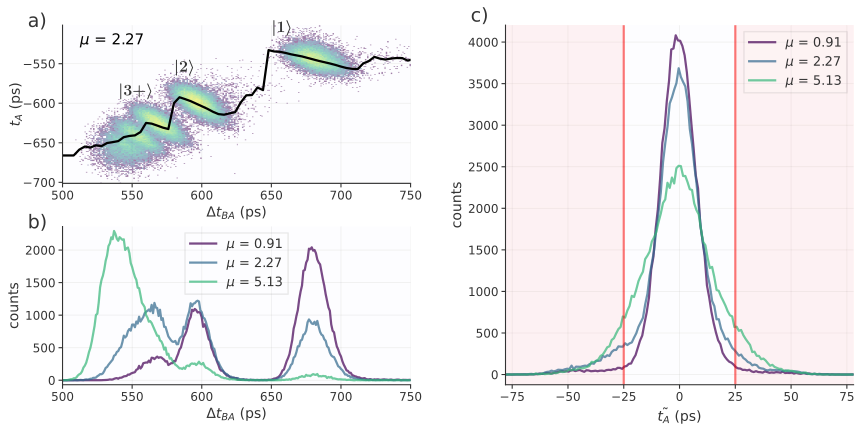
\includegraphics[width=1\textwidth,height=\textheight]{./chapter_04/figs/slope_cancellation_light.svg}
\caption[{PNR Slope Variation Analysis and Cancellation}]{\textbf{PNR Slope Variation Analysis and Cancellation} a) 2D histogram of RF pulse measurements. Through graphing slope $\Delta t_{BA}$ on the x-axis and arrival time $t_A$ on the y-axis, a series of groupings are visible that identify the discrete photon numbers detected.}
\label{fig:slope_correction}
\end{figure}
}

Pairs of pulse measurements $t_A$ and $t_B$ may be graphed on a 2D plane parametrized by $\Delta t_{BA}$ on the x-axis and $t_A$. Fig.~\ref{fig:slope_correction} a shows how this protection exhibits multiple groupings that correspond the the photon number character of the impinging optical mode. The 1 and 2-photon events are clearly identifiable and seperated from other events, with $|3\rangle$, $|4\rangle$, and $|5\rangle$ events also visible with less mutual separation. While Fig.~\ref{fig:slope_correction} a is shown here for just one mean photon number $\mu$, these grouplings are collected for a full range of attenuations and corresponding $\mu$. Fig.~\ref{fig:slope_correction} a shows histograms from projecting 3 such groupings down onto the $\Delta t_{BA}$ axis.

Thee slope correction method involves the measurement and creation of a slope-versus-arrival time line, one of which is shown in Fig.~\ref{fig:slope_correction} a. This is produced by averaging all $t_A$ measurements for a given slope $\Delta t_{BA}$. That is, the values along vertical slices of the 2D density plot in Fig.~\ref{fig:slope_correction} a are averaged to produce the y-coordinates of the slope-versus-arrival time line shown in black. By interpolating new $\Delta t_{BA}$ measurements on this curve and using it like a lookup table, PNR corrections $C_A$ are found. These may be subtracted off from $t_A$ producting $\tilde{t_A} = t_A - C_A(\Delta t_{BA})$ where $\tilde{t_A}$ is a constructed timing measurement that exhibits a symmetric arrival time response function and shown in Fig.~\ref{fig:slope_correction} c.~

The data representation and calibration curve shown in Fig.~\ref{fig:slope_correction} a may be constructed with $t_B$ on the y-axis as well. Then the PNR corrections are applied the the $t_B$ measurements instead. However, the resulting histograms $\tilde{t_B}$ are virtual identical to $\tilde{t_A}$.

\hypertarget{cluster-analysis}{%
\subsection{Cluster Analysis}\label{cluster-analysis}}

\hypertarget{results}{%
\section{Results}\label{results}}

results here

{}

\hypertarget{synchronization-with-a-software-phase-locked-loop-pll}{%
\section{Synchronization with a Software Phase Locked Loop (PLL)}\label{synchronization-with-a-software-phase-locked-loop-pll}}

\textbf{Todo}
\emph{This will be the first place in the thesis that I introduce the use of my software based phase locked loop (PLL). The software PLL has been useful in several later projects. I will either fully explain the PLL here, or I will only introduce and motivate it here. And a full description will go in an appendix. }
1. For sending many PPM symbols, I needed a synchronization clock that was (A) always running, and (B) extremely low jitter.
2. Sending an output from the AWG to the Swabian timetagger in another room resulted in a less-than-ideal clock source. The signal was low amplitude, and triggering on it's rising edge did not make for a very low jitter clock signal.
3. I had some sense that that should be a way of `averaging' past clock cycles in some way to cancel jitter. After some research and failed tests toward developing my own averaging method, I learned a software based Phase Locked Loop is just what I needed.
4. Initial version was adapted from a Matlab code on the Phase Locked Loop wikipedia page. That code was written for a sampled sign wave, but I adapted to take in just one data point per period. For our non-coherent and time-resolved types of measurements with SNSPDs, we typically only have clocks of this type. Where the clock is expressed by some type of optical or RF pulse that arrives on a regular period.
5. More recently Rahaf Youssef and I have worked on updating our software PLL tools so that its easier to understand and reason about, and easier to lock to a given signal.

\hypertarget{outlook-towards-high-rate-pnr-and-time-walk-correction}{%
\section{Outlook: Towards High Rate PNR and Time Walk Correction}\label{outlook-towards-high-rate-pnr-and-time-walk-correction}}

\hypertarget{high-rate-entanglement-generation}{%
\chapter{High Rate Entanglement Generation}\label{high-rate-entanglement-generation}}

A version of this chapter is currently under review. A preprint is released as:

Andrew Mueller, Samantha Davis, Boris Korzh, Raju Valivarthi, Andrew D. Beyer, Rahaf Youssef, Neil Sinclair, Matthew D. Shaw, \& Maria Spiropulu. (2023). \href{https://arxiv.org/abs/2310.01804}{High-rate multiplexed entanglement source based on time-bin qubits for advanced quantum networks}.

\hypertarget{abstract-3}{%
\section{Abstract}\label{abstract-3}}

Entanglement distribution based on time-bins is an attractive option for emerging quantum networks. We demonstrate a 4 GHz repetition rate source of photon pairs entangled across early and late time bins separated by 80 ps. Simultaneous high rates and high fidelities are achieved through multiplexing the Spontaneous Parametric Down Conversion (SPDC) output into 8 energy-time entangled channel pairs. We demonstrate entanglement fidelities as high as 99.76\%, total entanglement rates up to 0.5 Mbits/s, and predict a straightforward path towards achieving up to {\color{darkred} XXX} Mbit/s. Finally, we resolve the density matrices of individual channels and express distillable entanglement rates in ebit/s, thereby quantifying the tradeoff between fidelity and coincidence rates that contributes to useful entanglement distribution. This source is a fundamental building block for high rate entanglement-based quantum key distribution systems or advanced quantum networks.

\hypertarget{introduction-4}{%
\section{Introduction}\label{introduction-4}}

~~~~~

Entangled photons play a vital role in the development of quantum information processing and communication systems. The ability to generate entangled photon pairs at a high rate is essential for establishing reliable and scalable quantum networks, as well as for implementing entanglement-based quantum key distribution (QKD) systems. Unlike QKD systems that rely on attenuated lasers, entanglement distribution systems may fulfill the objectives of QKD while also serving as the foundation for advanced quantum networks that heavily rely on entanglement as a fundamental resource.

Entanglement-distribution and entanglement-based QKD systems have been demonstrated with impressive performance across a number of metrics. These include 40 Kbps data rates in a QKD system deployed over 50 km of fiber \autocite{Pelet2022}, as well as multiple polarization entangled sources that leverage spectral multiplexing. These polarization sources include a demonstration of 181 kebits/s across 150 ITU channel pairs, and a high-power source potentially capable of gigabit rates with many added channels and detectors \autocite{Alshowkan2022,Neumann2022Entanglement}. Multiple works have highlighted the need to leverage high total brightness, spectral brightness, collection efficiency, and high visibility from pair generating non-linear crystals in order to realize practical high-rate entanglement distribution \autocite{Neumann2022Entanglement}.

Also, with suitable equipment, robust time-bin modulation is possible over free space links with turbulence \autocite{Jin2019}. Therefore, the possibility of simplified fiber-free space interconnects and larger quantum networks based on a shared time-bin protocol motivates development of improved time-bin sources.

We employ a 4.0 GHz mode locked laser source with 80-ps delay interferometers to realize a high-rate source. Wavelength multiplexing is used for reading out energy-time entangled photon pairs, thereby realizing multiple high fidelity channels pairings which together sum to a high coincidence rate. Each of the 8 pairs can be considered an independent carrier of photonic entanglement \autocite{Wengerowsky2018} and therefore the system as a whole is applicable to flex-grid architectures through the use of wavelength selective switching \autocite{Appas2021,Alshowkan22Switching}. However, we focus here on maximizing the rate between two receiving stations, Alice and Bob (Fig.~\ref{fig:system} a). Each station is equipped with DWDMs that receive multiplexed channels, and may include multiple detectors to read out the full rate.

\hypertarget{fig:system}{%
\begin{figure}
\centering
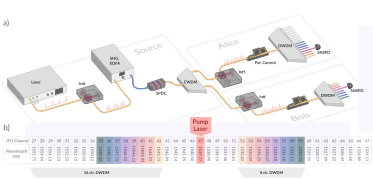
\includegraphics[width=1\textwidth,height=\textheight]{./chapter_05/figs/sys_drawing_light.svg}
\caption[{System Drawing \& DWDM Channels.}]{\textbf{System Drawing \& DWDM Channels} a) Pulses from a 1539.47 nm mode locked laser (Pritel UOC) are doubled by an 80 ps delay interferometer before up-conversion and amplification in a SHG \& EDFA module (Pritel). A short PM fiber from the SHG connects to the SPDC where photon pairs are created. The CWDM module separates the SPDC spectrum into multiple $\sim\!\!13~\mathrm{nm}$ wide bands spaced by 20 nm. The 1530 and 1550 nm bands are sent to the Bob and Alice stations respectively. The readout interferometers have the same time delay as the source interferometer. Polarization controllers are used to maximize the coincidence rates, as the detection efficiencies of the SNSPDs is polarization sensitive $\pm20\%$. Entanglement fidelity is unaffected by readout polarization. The two SNSPDs are connected to each channel pair in succession to resolve full system performance. b) ITU channels involved with the experiment. Pairs of channels highlighted with the same color obey the SPDC \& pump energy matching condition, and can be directly read out through DWDM channel outputs. To asses the full 16 channels (27-42) of Alice's DWDM multiplexer, Bob's 8-channel DWDM is switched out for a tunable narroband filter.}
\label{fig:system}
\end{figure}
}

We quantify per-channel brightness and fidelity as a function of pump power, as well as collection efficiencies, coincidence rates across 8 channel pairs, and expected performance of a partially realized 16-channel pair configuration. We show that the 8 channel system achieves low-power fidelities that average to 99.76\%. At a higher power, we demonstrate a total coincidence rate of 0.51 MHz with fidelities that average to 99.22\%. Through quantum state tomography we bound the distillable entanglement rate of the system to between 80\% and 95\% of the high-power coincidence rate (0.41 - 0.48 Mebits/s).

Quantifying a source's spectral mode purity is important for gauging its utility in advanced quantum networks that rely on 2-photon interference measurements like Bell State Measurements.

With Schmidt decomposition we quantify the modal purity of single DWDM channel pairs and derive the inverse Shmidt number which serves as an estimate for two-photon HOM visibility between two such sources. Ultimately, we demonstrate that an entanglement generation source of this design makes for a robust and powerful building block for future high rate quantum networks.

\hypertarget{system}{%
\section{System}\label{system}}

Figure \href{./section_03_introduction.md\#fig:system}{system} shows the experiment setup. Pulses from a 4 GHz mode locked laser (Pritel UOC) with a center wavelength at 1539.47 nm are sent through an 80 ps delay interferometer (Optoplex). This generates the early/late basis, which is subsequently unconverted by a second harmonic generation (SHG) module (Pritel) and down converted into entangled photon pairs by a type-0 spontaneous parametric down conversion crystal (Covesion). The up-converted pulses at 769 nm have a FWHM bandwidth of 243 GHz (0.48 nm), which along with the phase matching condition of the SPDC waveguide, defines a wide Joint Spectral Intensity (JSI) function.

The entangled pairs, which are separated by a coarse wavelength division multiplexer (CWDM), are of the form $|\psi\rangle=\frac{1}{\sqrt{2}}\left(|1\rangle_{s}|1\rangle_{i}+e^{i \phi}|2\rangle_{s}|2\rangle_{i}\right)$. Entangled idler and signal photons are sent to the receiving stations labeled Alice and Bob. One readout interferometer at each station projects all spectral bands into a composite time-phase basis. From here, dense wavelength division multiplexers (DWDM) divide up the energy-time entangled photon pairs into spectral channels.

The outputs of the DWDMS are sent to differential niobium nitride (NbN) superconducting nanowire single photon detectors (SNSPDs) \autocite{Colangelo2023} with efficiencies of \textcolor{red}{XX} and \textcolor{red}{XX}. These measure the arrival time of photons with respect to a clock signal derived from the mode locked laser. We use two SNSPDs for this demonstration, but a full 8-channel implementation of this system requires 16 detectors operating in parallel at both Alice and Bob. To read out both outputs of both interferometers, 4 detectors per channel are required.

\hypertarget{results-1}{%
\section{Results}\label{results-1}}

The JSI is measured in Fig. Fig.~\ref{fig:jsi} a by recording coincidence rates for different ITU channel pairings. For a given idler photon wavelength, the spectrum of corresponding signal photons spans several ITU channels. Pairs along the main diagonal are optimized for maximum coincidence rates, and are therefore used for all remaining measurements. In \href{./section_03_introduction.md\#fig:system}{system} c, these pairs are highlighted with matching colors.

\hypertarget{fig:jsi}{%
\begin{figure}
\centering
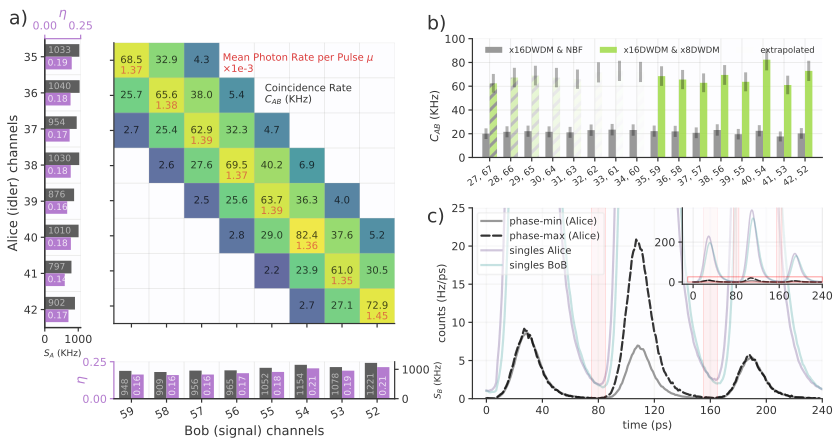
\includegraphics[width=1\textwidth,height=\textheight]{./chapter_05/figs/jsi_figure_light.svg}
\caption[{Channel JSI and Histogram.}]{\textbf{Channel JSI and Histogram} a) The singles rates $S_A$ and $S_B$ (grey bars), coupling efficiencies (purple bars), and coincidence rates $C_{AB}$ (diagonal boxes) for different DWDM channel pairings. The joint spectral intensity envelop spans several 100 GHz channels. So the coincidence rates (KHz, in black) are consistent with the efficiencies $\eta$ (purple bars) and the singles rates (grey bars), they are scaled to represent two branches of the total wavefunction. There are four branches in all, for the 4 pairs of 2 interferometer output ports that contribute coincidences. In practice, one output each of Alice and Bob's interferometers is measured, thereby capturing one branch. See supplemental for details of the scaling method, and the fitting method used to solve for the coupling efficiencies $\eta$. b) Coincidence rates for energy-matched channel pairings. The light green bars match the main diagonal in (a). Grey bars are measured with x16 DWDM at Alice and a tunable narroband filter at Bob. Dashed bars predict the rates for a system with x16 DWDMs at both Alice and Bob c) Histogram of photon arrival events with respect to the 4 GHz clock. Dashed black and grey lines show the response functions for coincidence events. Red bars represent guard regions where coincidence events are ignored.}
\label{fig:jsi}
\end{figure}
}

Figure Fig.~\ref{fig:jsi} a also shows coupling efficiencies $\eta$ for each DWDM channel, $S_A$ is the singles rate at Alice, and $S_B$ is the singles rate at Bob \autocite{Neumann2022Entanglement}. As only two of the total four interferometer output ports are measured at once, certain scalings are made to the singles and coincidence rates $C_{AB}$ to reflect a readout configuration with well defined coupling efficiency (see supplementary information).

Most tests were done with the 8 ITU 100 GHz channel pairings: Ch. 35-42 at Alice and Ch. 52-49 at Bob. In Fig. Fig.~\ref{fig:jsi} b we investigate rates across 16 pairs by using all 16 channels available on the DWDM at Alice (24 - 34) and a tuneable narroband filter in place of the DWDM at Bob. As the narroband filter has higher loss, the coincidence rates are lower (grey bars in Fig. Fig.~\ref{fig:jsi} b). But the uniformity of coincidence rates across 16 channels implies the use of 16-channel DWDMs at both Alice and Bob would roughly double the total coincidence rate.

Signals from the SNSPDs are read out with a free running time tagger (Swabian) and processed with custom software. In the resulting histograms referenced from a shared clock (Fig Fig.~\ref{fig:jsi} c), three peaks are visible which are caused by the sequential delays of the source and readout interferometers. Some intensity imbalance between long and short paths is present in these interferometers, which explains the asymmetry between early and late peaks in Fig.~\ref{fig:jsi} c.~This type of imbalance is expected to degrade entanglement fidelity only if present in the source interferometer (see supplemenatry info). Therefore, that with lowest imbalance was chosen for the source.

The coincidence rate across Alice and Bob's middle bins varies sinusoidally with respect to the combined phase relationship source and readout interferometers (see supplementary information) \autocite{Inagaki2013}. In figure Fig.~\ref{fig:jsi} c the coincidences shown are for any combination of early, middle, or late bins. For tomography and fidelity measurements, coincidences across specific bin pairings are considered. Events within 10 ps width guard regions centered at 80 and 160 ps (shaded red) are discarded for analysis of coincidences between individual bins. This is done to maximize fidelity in the presence of some minor overlap of the pulse response functions.

\hypertarget{fig:shg_scan}{%
\begin{figure}
\centering
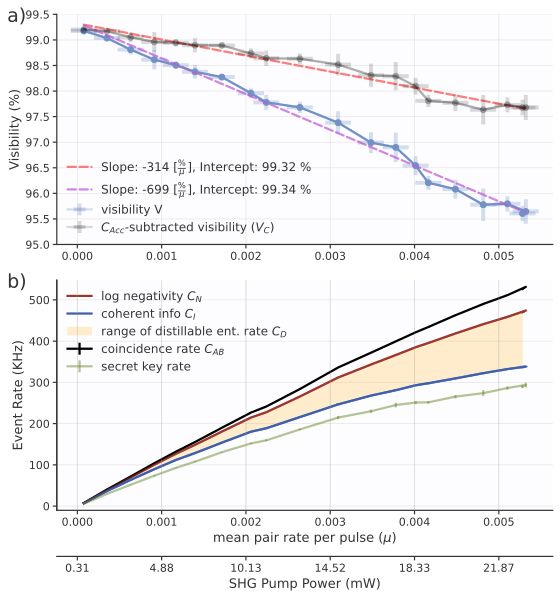
\includegraphics[width=1\textwidth,height=\textheight]{./chapter_05/figs/shg_scan_light.svg}
\caption[{Fidelity and Rates vs \(\boldsymbol \mu\).}]{\textbf{Fidelity and Rates vs $\boldsymbol \mu$} a) Fidelity versus pump power. Error bars arise from making multiple measurements of the center bin coincidence rate over some integration time. These measurements span small ranges of interferometer phase, as the extremum-finding algorithm jitters the interferometer voltage. b) Bounded distillable entanglement rate versus pump power. Multiple such measurements are made for all the tomographic measurements. These are used to calculate standard deviations for fidelity, log negativity, and coherent information. Error bars for the log negativity and coherent information are smaller than the line width shown. Rates shown assume readout of all 4 available interferometer ports, based on data measured using one port each at Alice and Bob.}
\label{fig:shg_scan}
\end{figure}
}

Due to the small size and athermal design of the interferomters, minimal temporal phase drift was observed over multiple hours. Nevertheless, software was used to `lock' the phase at a minimum or maximum with a simple steepest-descent algorithm. This varied the phase by small amounts over several minutes and adjusted phase to maintain an extremum.

Channels 35 and 59 were chosen for an analysis of entanglement fidelity and rates versus pump power. Fidelity with respect to pump power or mean entangled pair rate is shown in Fig.~\ref{fig:shg_scan} a. We define the entanglement fidelity as $F = 100\%*(1 - \frac{C_{min}}{C_{max}})$ where $C_{min}$ and $C_{max}$ are the minimum and maximum coincidence rates with respect to interferometer phase observed across the middle bins. As this coincidence rate depends on the total phase across all source and readout interferometers, just one (Bob's) is actively controlled to scan the full state space.

\hypertarget{fig:channel_data}{%
\begin{figure}
\centering
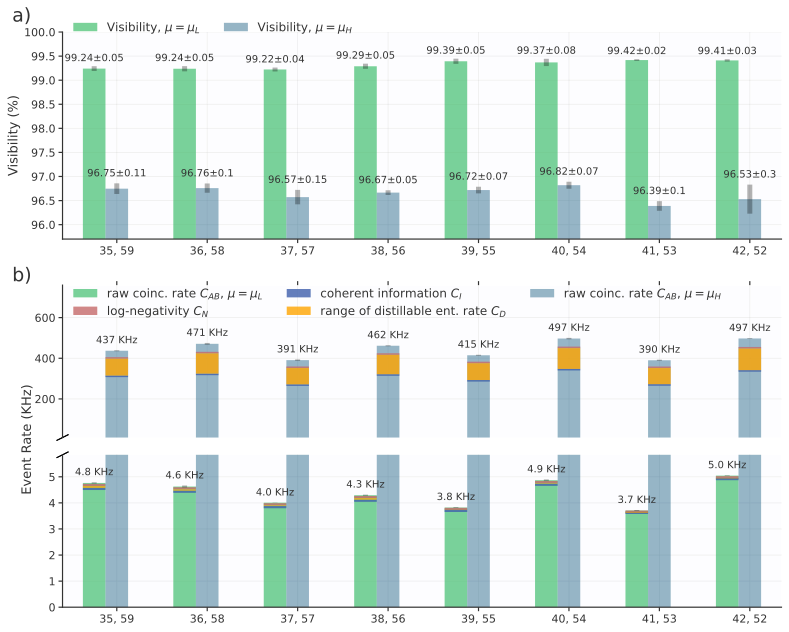
\includegraphics[width=1\textwidth,height=\textheight]{./chapter_05/figs/8ch_bar_graph_high_power_light.svg}
\caption[{Fidelity and rates across 8 channel pairs.}]{\textbf{Fidelity and rates across 8 channel pairs} a) Fidelity for the main 8 channel pairs, measured at a high (5.17 Amps) and a low ( 1.2 Amps) SHG pump power setting. Each power setting results in similar $\mu$ for all channels: $\mu_{low}$ = 5.6e-5 $\pm$ 9e-6 and $\mu_{high}$ = 6.1e-3 $\pm$ 3e-4. b) Rate metrics for the 8 channel pairs at the same high and low power settings. The range of possible values for distillable entanglement rate is spanned by the yellow regions, bounded above by log-negativity and below by coherent information. Rates shown assume readout of all 4 available interferometer ports, based on data measured using one port each at Alice and Bob}
\label{fig:channel_data}
\end{figure}
}

We quantify the rate of useful entanglement by supplying bounds for the distillable entanglement rate $R_D$. Measured in ebits/s, $R_D$ is the maximal asymptotic rate of Bell pair production per received state using only local operations and classical communications. It is bounded above by log negativity $R_N = RE_N$ and below by $R_I = R E_I$ where $R$ is the raw coincidence rate \autocite{Alshowkan2022}. For each pump power setting in Fig.~\ref{fig:shg_scan}, a series of tomographic measurements is performed and density matrices calculated. $E_I$ and $E_N$ are calculated from the density matrices as detailed in the supplementary information.

Figure Fig.~\ref{fig:channel_data} shows fidelities, raw coincidence rates, and bounded distillable entanglement rates for all 8 channel pairings and 2 pump powers. The higher pump power is the highest possible on our SHG \& EDFA module. Higher rates are readily achievable by increasing the output power of this component, up to a point where the high count rate on the SNSPDs induces higher jitter. However these pulse pileup and time-walk effects can be mitigated with jitter correction techniques \autocite{Mueller2023}.

\% \textbackslash textcolor\{blue\}\{
\% We perform a linear fit of the entanglement fidelity data, $F = A + B\mu$, and obtain $A = XXX$, $B=XXX$. We derive expressions for A and B in terms of the mean photon number, interferometer transmittances, and interference visibilities (see Supplemental).\}

Using the data in Fig. Fig.~\ref{fig:jsi} a, we model the joint spectral intensity function of the SPDC output as a product of pump envelope and phase matching condition functions

$$|f(\omega_s, \omega_i)|^2 = |\psi_{\mathrm{ph}}\left(\omega_s, \omega_i\right)|^2 *|\psi_p\left(\omega_s, \omega_i\right)|^2$$

This construction depends on the wavelength (769.78 nm) and bandwidth (243 GHz FWHM) of unconverted light out of the SHG, which was measured with a spectrum analyzer. The transmission spectrums of the 100 GHz DWDM channels was also modeled based on measured transmission data, in order to define the integrations over the JSI that would match the coincidence results in Fig. Fig.~\ref{fig:jsi} a (details in supplemental).

We calculate the Schmidt decomposition of the JSI bipartite spectrum transmitted through pairs of DWDM filters at Alice and Bob, and derive an inverse Schmidt number of $1/K = 0.87$. This value quantifies the spectral purity of the entangled photon source, and predicts the visibility of a two-source HOM (Hong-Ou-Mandel) interferogram. If 50 GHz ITU channels are used instead, the model predicts $1/K = 0.96$.

\hypertarget{conclusion}{%
\chapter{Conclusion}\label{conclusion}}

\appendix

\hypertarget{aph-138-homework-assignment}{%
\chapter{Aph 138 Homework Assignment}\label{aph-138-homework-assignment}}

In March of 2022, Matthew Shaw was a guest lecturer for the Quantum Hardware and Techniques course (APh/Ph 138b). The following is a homework assignment I wrote to accompany his series of lectures.

The first problem is inspired by the low dark count rate publication~\autocite{Mueller:21}. It has the student build a simple model for a dark count rate transmitted through a series of filters. Finally, it leads the student to consider an ultimate tradeoff between dark count rate and coupling efficiency to wide bandwidth optical signals. A filtering system that only transmits a very narroband signal will not be able to detect ultra-short optical signals with high efficiency or temporal resolution.

The second problem explores a potential use case of a photon number resolving SNSPD. It closely follows logic presented in an Andreas Christ and Christine Silberhorn paper~\autocite{Andreas:12}. I studied this paper earlier in my PhD, when I considered developing a multiplexed single photon source. It turned out that project was overly ambitious, but future PhD students might consider approaching it again.

\textcolor{midnightblue}{Contact \href{mailto:andrewstermueller@gmail.com}{Andrew Mueller} with any questions about the homework or solution manual. The solutions to some sections specify finer-grained point values when there are multiple answers per section. As the grader, feel free to use these or not. }

\hypertarget{free-space-coupling-with-low-dark-counts-50-points}{%
\subsection{1. Free space coupling with low dark counts (50 points)}\label{free-space-coupling-with-low-dark-counts-50-points}}

An experimental apparatus emits a collimated beam of $1550~\mathrm{nm}$ photons with gaussian beam waist $w_0 = 3~\mathrm{mm}$. You wish to focus the beam onto an SNSPD directly through a window in a cryostat.

\hypertarget{fig:cryostat_concept}{%
\begin{figure}
\centering
\includegraphics{./chapter_07/figs/fig1b_light.svg}
\caption[{Cryostat optical coupling}]{\textbf{Cryostat free space coupling options.}}
\label{fig:cryostat_concept}
\end{figure}
}

As we will see later on, a set of filters will be needed between the detector and the window to minimize dark counts. In practice, the set of filters can be quite thick. Say a $f = 100~\mathrm{mm}$ lens is used right outside the cryostat to focus the beam onto the detector though a set of filters (Fig.~\ref{fig:cryostat_concept} a). The long focal length makes room for a few inches of filters between the external lens and focused spot.

\begin{enumerate}
\def\labelenumi{\arabic{enumi}.}
\item
  (4 pts)
  If the detector has a circular active area with radius $5~\mathrm{\upmu m}$, what ratio of power in the beam can it collect? Assume the detector has unity efficiency across all angles of incidence with respect to the surface normal.

  \textcolor{midnightblue}{

  \textbf{Answer:}

  }

  \textcolor{midnightblue}{

  The divergence angle of the guassian beam: $\theta = \tan^{-1}({\frac{3}{100}})$.

  }

  \textcolor{midnightblue}{ The formula for divergence angle in terms of waist $w_0$: $\theta = \frac{\lambda}{\pi w_0}$ }

  \textcolor{midnightblue}{ Combining and plugging in, the waist radius at focus is $\frac{1550~\mathrm{nm}}{\pi \tan^{-1}(\frac{3}{100})} \approx 16.5~ \mathrm{\upmu m}$ }

  \textcolor{midnightblue}{ The formula for power inside an aperture at $w(z)$ for a guassian beam:}

  \textcolor{midnightblue}{

  $$P(r, z)=P_{0}\left[1-e^{-2 r^{2} / w^{2}(z)}\right]$$

  }

  \textcolor{midnightblue}{We are interested in the ratio of power collected at $w(z=0) = w_0$ which may be expressed as:}

  \textcolor{midnightblue}{

  $$P(r, z=0)=1-e^{-2 r^{2} / w_0^{2}}$$

  }

  \textcolor{midnightblue}{Plugging in: }

  \textcolor{midnightblue}{

  $$P(r, z=0)=1-e^{-2(5^{2}) / 16.5^{2}} \approx  \boxed{0.17} $$

  }
\item
  (4 pts)
  A faster lens mounted much closer to the detector inside the cryostat focuses to a smaller waist. Consider an $f = 18~\mathrm{mm}$ lens with the detector at the focal length (Fig.~\ref{fig:cryostat_concept} b). Verify more than 99\% of the collimated light will be focused onto the active area of the detector.

  \textcolor{midnightblue}{ The waist radius at focus is $\frac{1550~\mathrm{nm}}{\pi \tan^{-1}(\frac{3}{18})} \approx 2.98~\mathrm{\upmu m}$ }

  \textcolor{midnightblue}{Ratio of power within the $10~\mathrm{\upmu m}$ radius active area: }

  \textcolor{midnightblue}{

  $$P(r, z=0)=1-e^{-2(5^{2}) / 2.98^{2}} \approx \boxed{0.996} $$

  }

  Without filtering, the mid-infrared photons coupled to the detector from the room temperature laboratory are a dominant source of dark counts. Think of the environment outside the window as an isotropic blackbody emitter. Consider 3 cases, where the shaded red regions illustrate the light field of thermal radiation that could couple to the detector:

  \hypertarget{fig:coupling_options}{%
  \begin{figure}
  \centering
  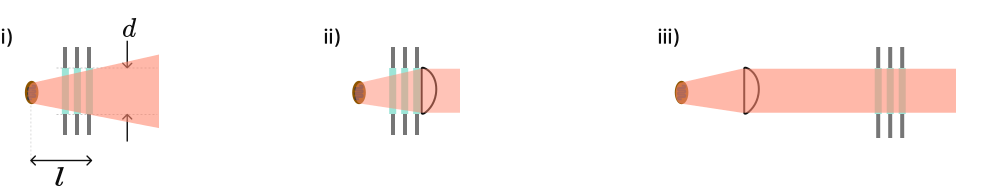
\includegraphics{./chapter_07/figs/fig2b_light.svg}
  \caption[{Cryostat coupling options}]{\textbf{Three Coupling Options}}
  \label{fig:coupling_options}
  \end{figure}
  }

  \begin{enumerate}
  \def\labelenumii{\roman{enumii})}
  \tightlist
  \item
    There is no lens; the detector is distance $l$ inside the cryostat, and the first window with diameter $d$ defines an entrance pupil.
  \item
    Same as (i), but a lens with focal length $l$ is placed right outside the first window. The detector is at the focal point.
  \item
    Same as (ii) but the lens is placed inside the cryostat with the detector still at the focal length. Equivalent to Fig.~\ref{fig:cryostat_concept} b above.
  \end{enumerate}
\item
  (6 pts) Does (ii) couple more, less, or equal dark counts to the detector than (i)? What about case (iii)? Why? No calculations should be needed.
  (Hint: Consider the units of radiance, which characterizes a black body emitter. Etendue or beam parameter product may be useful concepts to consider)

  \textcolor{midnightblue}{ \textbf{Answer:} }
  \textcolor{midnightblue}{ The three cases couple the same amount of light to the detector. (ii) couples the same amount of power as (i) because a blackbody source can't be focused to higher intensity with a lens. The solid angle subtended by the entrance pupil as seen by the detector is the same in all cases. The detector area stays the same as well so the etendue is conserved across all three cases. This implies the same radiant power is coupled. }

  \textcolor{midnightblue}{ 3 points for saying all situations couple the same rate; 3 points for some explanation. }
\item
  (9 pts) Using Planck's law with laboratory temperature $T$ and the geometry of case (i) above, write an expression for spectral radiant flux (photons per unit wavelength) on the active area of a detector with radius $r$.

  \textcolor{midnightblue}{ \textbf{Answer:} }
  \textcolor{midnightblue}{The expression is a product of several factors:}

  \textcolor{midnightblue}{

  $$\text{Flux}[\lambda] = P \Omega D_{area} B_{\lambda}(\lambda, T)$$

  }

  \textcolor{midnightblue}{ Where $P = \frac{\lambda}{hc}$ is the number of photons per unit energy, $\Omega$ is the solid angle of blackbody radiation as seen by the detector, $D_{area} = \pi r^2$ is the area of the detector, and $B_{\lambda}$ is Planck's law. }
  \textcolor{midnightblue}{Planck's law:}

  \textcolor{midnightblue}{

  $$B_{\lambda}(\lambda, T)=\frac{2 h c^{2}}{\lambda^{5}} \frac{1}{e^{h c /\left(\lambda k_{\mathrm{B}} T\right)}-1}$$

  }

  \textcolor{midnightblue}{ $\Omega = \pi \sin{\theta^2}$, where $\theta = \tan^{-1}(\frac{(d/2)}{l})$ is the half angle of the field of view of blackbody radiation as seen by the detector. }

  \textcolor{midnightblue}{The full expression: }

  \textcolor{midnightblue}{

  $$\text{Flux}[\lambda] = \frac{\lambda \pi^2 r^2 \sin{\theta^2}}{hc} \frac{2 h c^{2}}{\lambda^{5}} \frac{1}{e^{h c /\left(\lambda k_{\mathrm{B}} T\right)}-1}, \,\,\,\,\,\,\,\,\,\,\,\theta = \tan^{-1}(\frac{(d/2)}{l})$$

  }

  \textcolor{midnightblue}{ Since the expression asked for can be written many ways, just verify the student has taken into account all the terms in equation (1) above, and has the correct expressions for} \textcolor{darkred}{$\Omega$ (3 pts), $\theta$ (3 pts), and P (3 pts).}
\item
  (6 pts) Consider the configuration in Fig. 1b). The detector has an internal quantum efficiency approximated by:

  $$\eta(\lambda) = \frac{1}{2}(1 - \text{erf}[\lambda - 3~\mathrm{\upmu m}]) $$

  $\lambda$ is measured in $\mathrm{\upmu m}$ and $\text{erf}()$ is the error function. Using your conclusions from (1.3) and expression from (1.4), write a formula $N_{photons}[\lambda]$ for the number of detectable dark counts with respect to $\lambda$, then numerically integrate it to find the dark count rate with no filtering. The laboratory temperature $T$ is 293 K, lens focal length $l$ is $18~\text{mm}$, detector radius $r$ is $5~\mathrm{\upmu m}$, and the diameter $d$ of all optics is 1 inch. The maximum count rate of this SNSPD is 10 MHz. Is the detector usable or overexposed?

  \textcolor{midnightblue}{ \textbf{Answer:} }
  \textcolor{midnightblue}{Use the expression from (1.4) and multiply it by the quantum efficiency function $\eta(\lambda)$ }

  \textcolor{midnightblue}{

  $$N_{photons}[\lambda] = P \Omega D_{area} \eta(\lambda) B_{\lambda}(\lambda, T=293)$$

  }

  \textcolor{midnightblue}{ Here is the function expressed in mathmatica and the solution to the integral: }

  \textcolor{midnightblue}{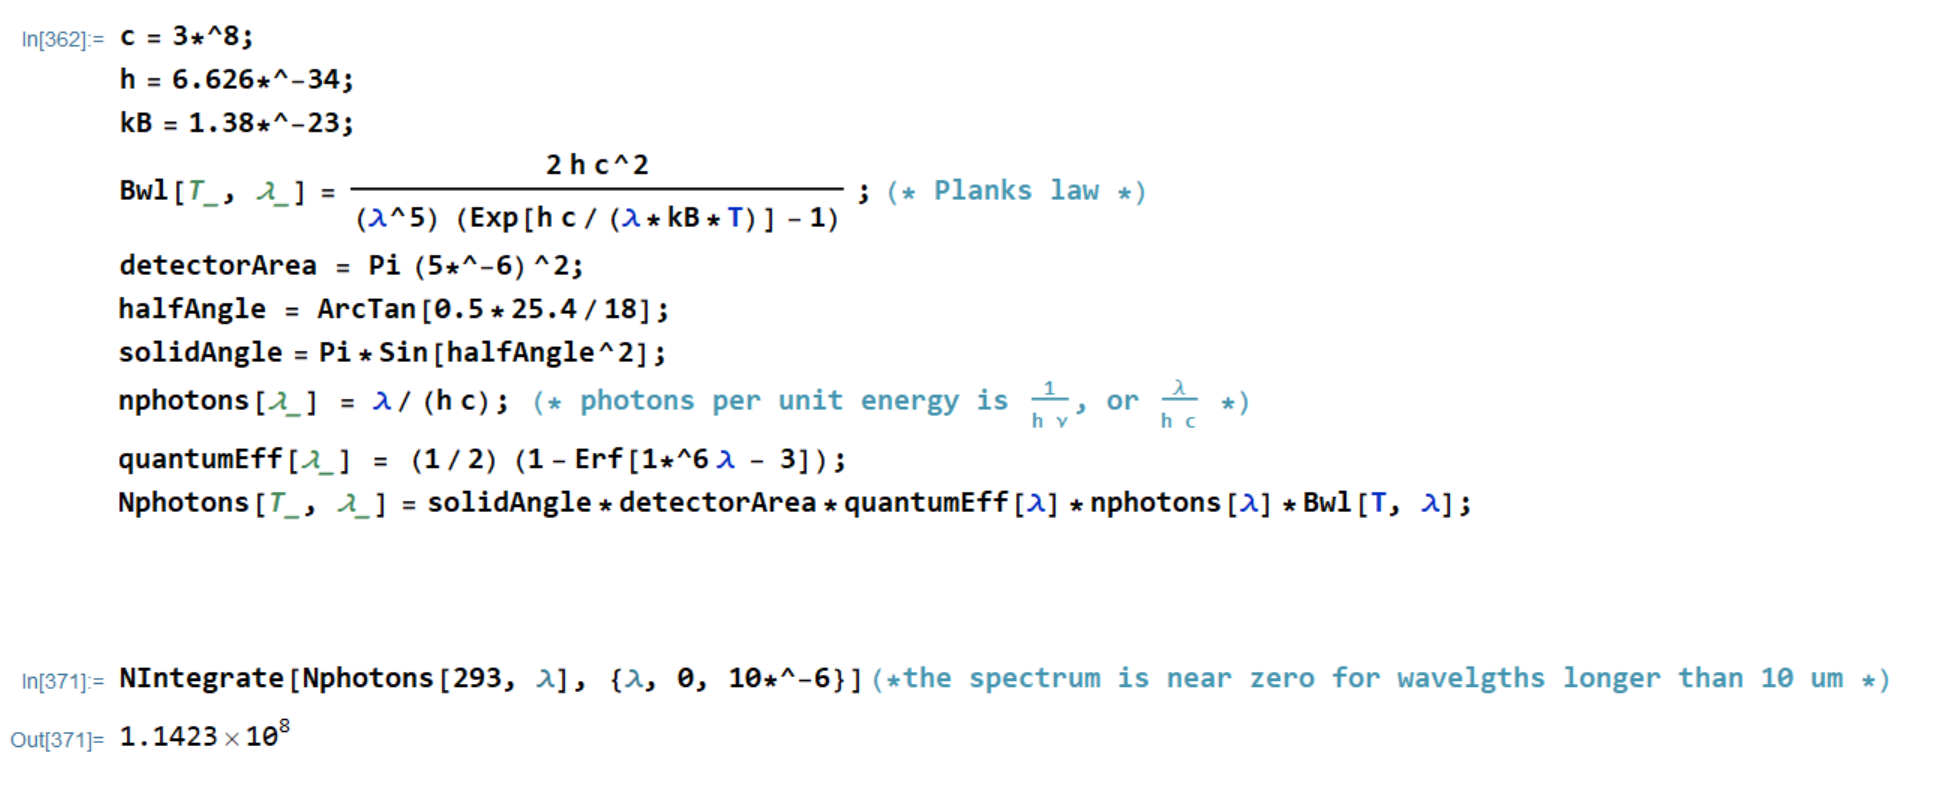
\includegraphics{./chapter_07/figs/mathematica_2.PNG}}

  \textcolor{midnightblue}{Dark count rate $\approx \boxed{110 \,\text{MCounts/s}}$ }
  \textcolor{midnightblue}{The rate of dark counts exceeds the usual maximum count rate, the detector is not usable. }

  \textcolor{midnightblue}{3 pts. for similar dark count rate (+/- 20\%) , 3 pts. for saying the detector is not usable.}
\item
  (6 pts) A set of shortpass filters can remove the bulk of blackbody radiation. A shortpass filter can be roughly modeled with the formula:

  $$F(\lambda, E_t) = \frac{1}{E_t}[(E_t - 1)H(\lambda_c - \lambda) + 1]$$

  Where H is the Heaviside step function, $\lambda_c$ is the cutoff wavelength of the filter, and $E_t$ is the extinction ratio of the filter. Use this with $N_{photons}[\lambda]$ from (d). How many filters with $\lambda_c = 1560~\text{nm}$ and $E_t = 30~\text{dB}$ are necessary to suppress the spectral region of detectable dark counts longer than 1560 nm so that it is not the dominant source of dark counts?

  \textcolor{midnightblue}{ \textbf{Answer:} }

  \textcolor{midnightblue}{$\boxed{\text{3 filters}}$ are needed to make the wavelength band shorter than 156 nm the dominant source of counts.} \textcolor{darkred}{3 pts. for this answer}

  \textcolor{darkred}{3 pts for evidence:}
  \textcolor{midnightblue}{Students might integrate the detectable dark count spectrum with different numbers of filters and comparing the results. The computations below show the addition of a fourth filter has a negligible effect on the dark count rate. }

  \textcolor{midnightblue}{Students may instead give a more qualitative answer, for example with a graph of the filtered spectrums, that shows the relative suppression of the region longer than 1560 nm. }

  \textcolor{midnightblue}{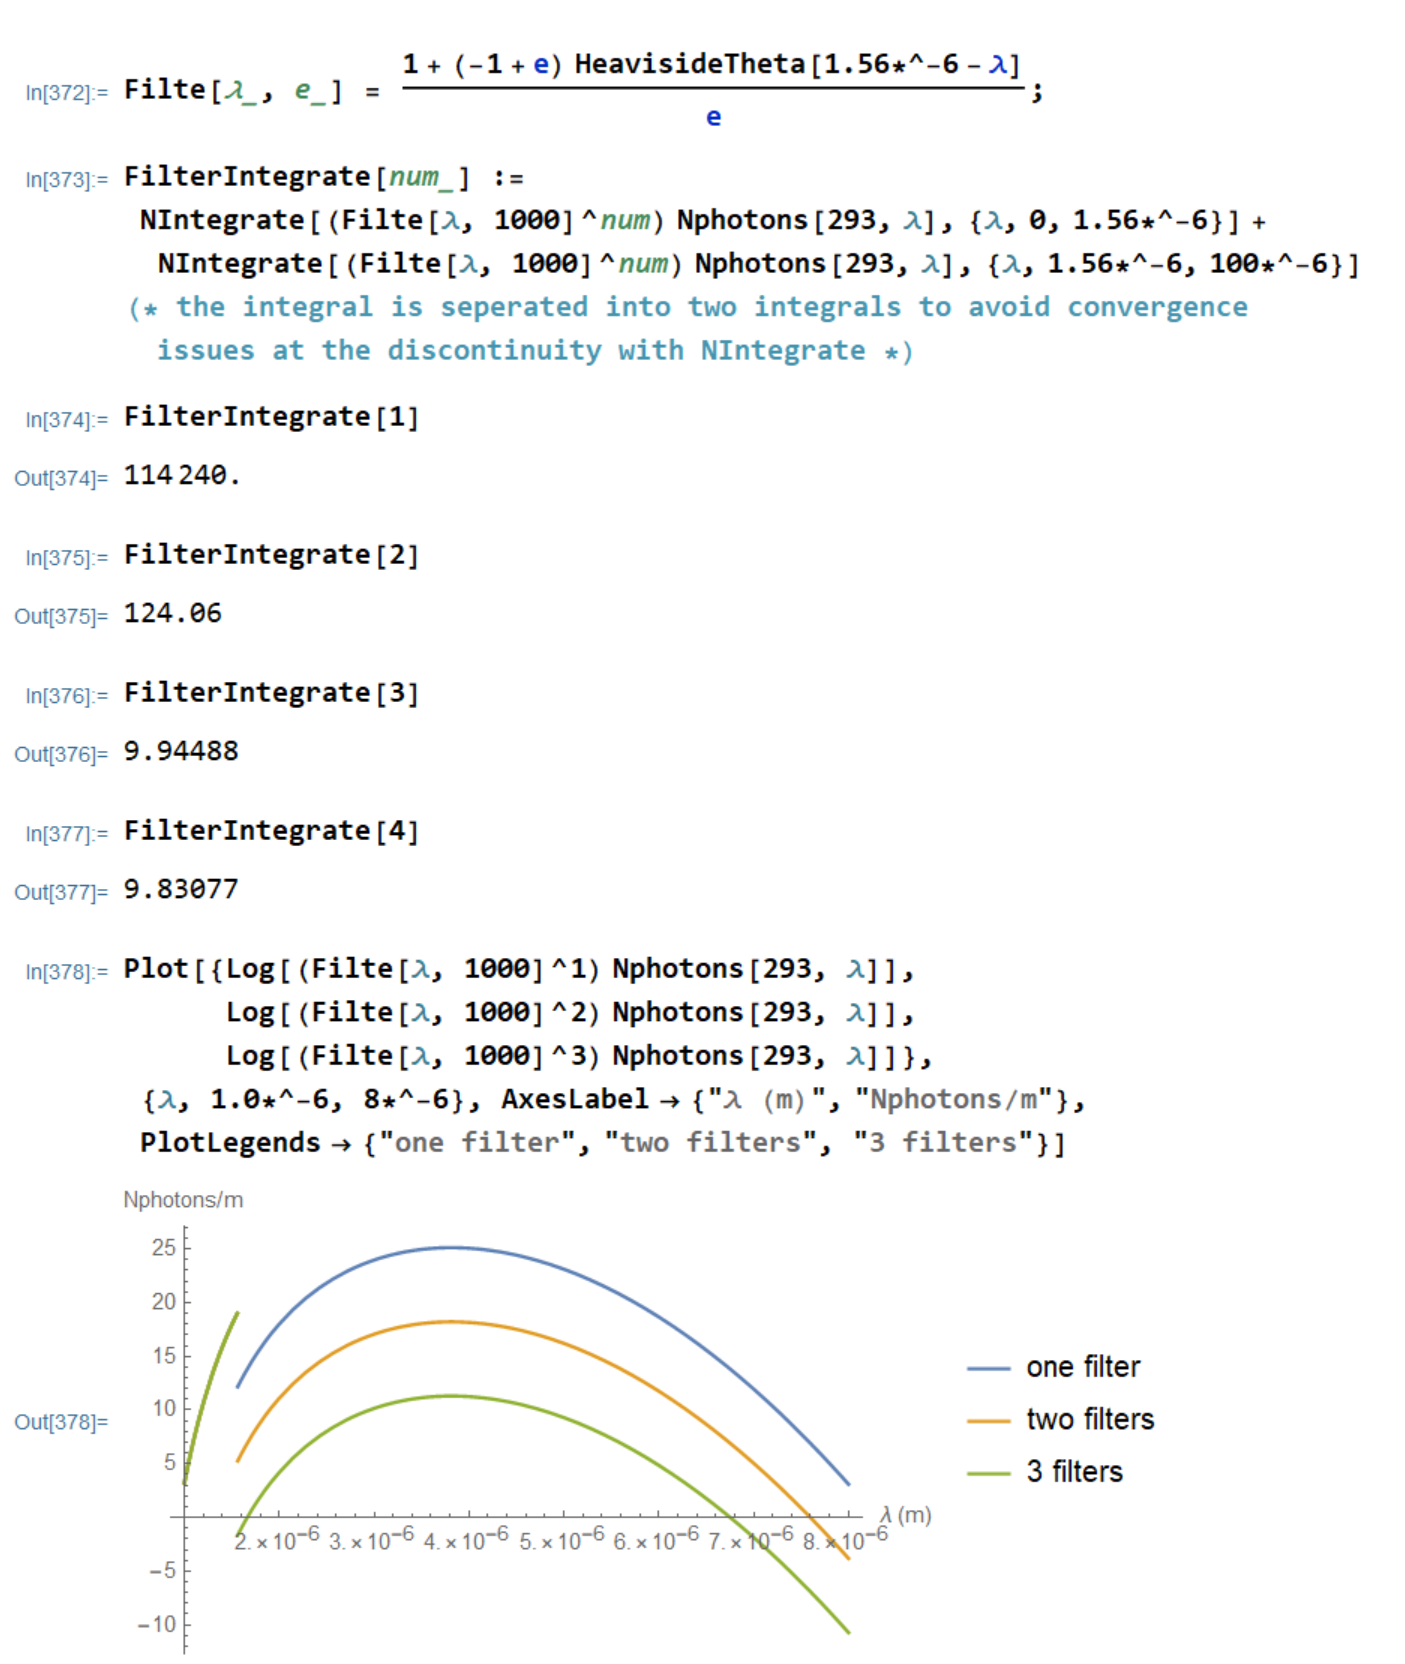
\includegraphics{./chapter_07/figs/filter_integrate_4.PNG}}
\item
  (7 pts) If a narrow band filter is also inserted with center wavelength $1550~\text{nm}$ and spectral width below $1-2~nm$, then dark count rate can be approximated as just $N_{photons}[\lambda = 1550~\text{nm}]$ times the filter width. Show for this wavelength range you can simplify dark count rate further to a simple exponential function. If the laboratory air conditioner breaks, raising the lab temperature from 293 K to 300 K, how much higher is the dark count rate?

  \textcolor{midnightblue}{ \textbf{Answer:} }

  \textcolor{midnightblue}{The expression for $N_{photons}[\lambda]$ from part (1.4) can be simplified and evaluated at 1550 nm, then multiplied by the filter width in nanometers. }

  \textcolor{midnightblue}{

  $$\begin{aligned}
   N_{photons}[\lambda] &= P \Omega D_{area} \eta(\lambda) B_{\lambda}(\lambda) \\
   N_{filter} &= N_{photons}[\lambda = 1550~\text{nm}]\Delta \lambda
   \end{aligned}$$

  }

  \textcolor{midnightblue}{This code shows integrating the spectrum and just multiplying $N_{photons}$ times the filter width produce very similar results (for a 1 nm filter):}

  \textcolor{midnightblue}{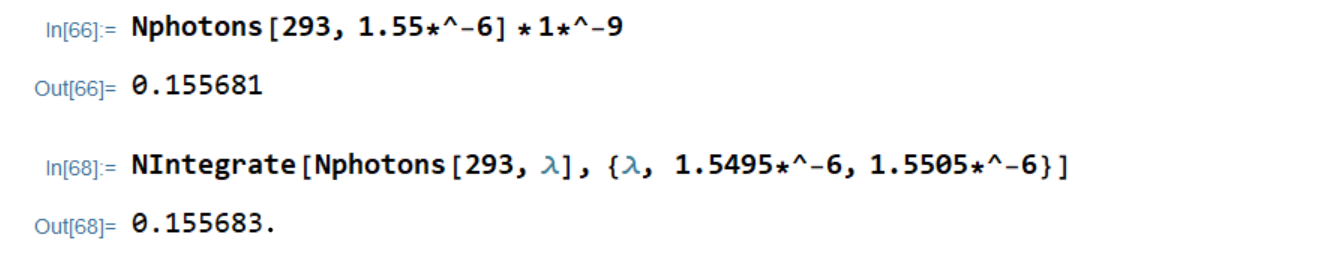
\includegraphics{./chapter_07/figs/nphoton_approx.PNG}}

  \textcolor{midnightblue}{Evaluating the $N_{photon}$ function at $\lambda = 1550~text{nm}$ shows the $-1$ term is small relative to the exponential term:}

  \textcolor{midnightblue}{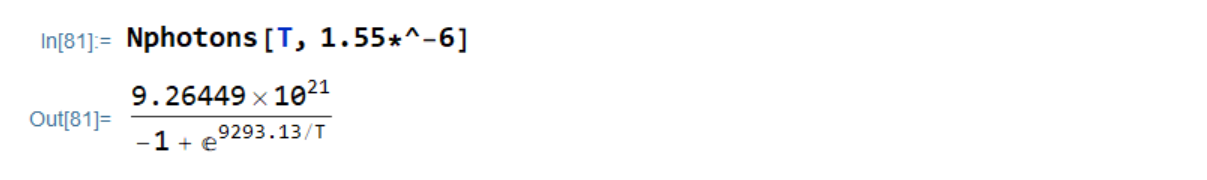
\includegraphics{./chapter_07/figs/small_relative_to_exponential.PNG}}

  \textcolor{midnightblue}{Therefore the filter transmission approximation is:}

  \textcolor{midnightblue}{

  $$\boxed{N_{filter} \approx 9.26\mathrm{e}21 \Delta\lambda e^{-9290/T} (\frac{\text{photons}}{\text{s*meter}})}$$

  }

  \textcolor{midnightblue}{or equivalently: }

  \textcolor{midnightblue}{

  $$\boxed{N_{filter} \approx 9.26\mathrm{e}12 \Delta\lambda e^{-9290/T} (\frac{\text{photons}}{\text{s*nm}})}$$

  }

  \textcolor{midnightblue}{and the dark count rate in the 300 K room is roughly double the rate in the 293 K room: }

  \textcolor{midnightblue}{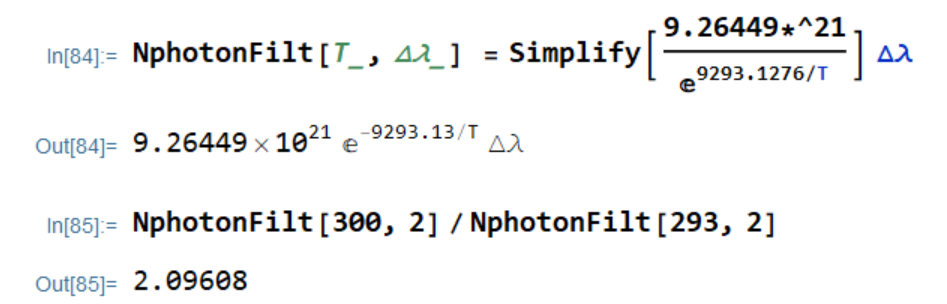
\includegraphics{./chapter_07/figs/filter_with_temp.PNG}}

  \textcolor{midnightblue}{4 pts for a similar equation, 3 pts for finding the dark count rate roughly doubles. }

  A quantum communication experiment requires time-tagging photons with respect to a 50 GHz clock with 95\% fidelity. That is, 95\% of the timing measurements of detected photons emitted at the same time with respect to a clock fall within a 20 ps bin. Say the detector and readout electronics have a combined jitter of 10 ps FWHM, and a mode locked laser is used for the experiment that generates transform-limited Gaussian pulses. You tune it's temporal length to a value for which the total timing uncertainty of time-tagged photons --- including system jitter and pulse temporal length --- matches the 95 \% fidelity at 50 GHz requirement. Assume detector jitter has a Gaussian shape as well.
\item
  (8 pts) Find the spectral width of a filter that would transmit 95\% of the photons from the mode locked laser. What is the dark count rate with this filter, using the expression from (1.7) and T = 293 K?

  \textcolor{midnightblue}{ \textbf{Answer:} }

  \textcolor{midnightblue}{For transform limited guassian pulses, the product of temporal and spectral width at a FWHM level is \href{https://www.lasercalculator.com/transform-limited-pulse-calculator/}{about 0.441}. There's a derivation of this \href{https://www.physicsforums.com/threads/time-bandwidth-product-ideal-mode-locking.171404/post-1339948}{here}, but students don't need to show it. }

  \textcolor{midnightblue}{

  $$T B P_{\text {Gaussian }}=\frac{2 \log 2}{\pi} \approx 0.441$$

  }

  \textcolor{midnightblue}{ Since this uses the FWHM level, all the 95\% metrics need to be converted. About 95\% of the area under a guassian falls within $\pm 2 \sigma$. }

  \textcolor{midnightblue}{ Bound on total system timing uncertainty: $20~\text{ps}_{95\%} = (20/4)*2.35 = 11.75~\text{ps}_{FWHM}$ }

  \textcolor{midnightblue}{ The jitter of the detection system and the temporal width of the laser pulse $\Delta t$ should add in quadrature to match the bound: }

  \textcolor{midnightblue}{

  $$ 11.75~\text{ps}_{FWHM} = \sqrt{ \Delta t^2 + (10~\text{ps})^2}$$

  }

  \textcolor{midnightblue}{

  $$\begin{aligned}
   0.441 = \Delta t \Delta \nu \\
   \Delta \nu = 71~\text{GHz} \\
   \Delta \lambda = \frac{\lambda^2 \Delta \nu}{c} = 0.57~\text{nm} \\
   \end{aligned}$$

  }

  \textcolor{midnightblue}{ $0.57~\text{nm}$ is the spectral width of the laser pulse at the FWHM level. If this pulse passes through a tophat filter with width equal to the 95\% level of the laser pulse, then 95\% will be transmitted. }

  \textcolor{midnightblue}{Filter width: }

  \textcolor{midnightblue}{

  $$\Delta \lambda_{95\%} = \frac{4 \Delta \lambda}{2.35} \approx \boxed{1~\text{nm}} $$

  }

  \textcolor{midnightblue}{Dark count rate is easy to find using the expression from the previous section: }

  \textcolor{midnightblue}{

  $$\boxed{N_{filter} \approx 9.26e12 (1~\text{nm}) e^{-9290/T} (\frac{\text{photons}}{\text{s*nm}})} \approx 0.15~\text{photons/s} $$

  }

  \textcolor{midnightblue}{3 points for writing and solving the equation that matches the jitter bound to the quadrature sum }
  \textcolor{midnightblue}{5 points for correct filter width and dark count rate}
\end{enumerate}

\hypertarget{spdc-coupling-and-single-photon-sources-50-points}{%
\subsection{2. SPDC Coupling and Single Photon Sources (50 points)}\label{spdc-coupling-and-single-photon-sources-50-points}}

A Spontaneous Parametric Down Conversion (SPDC) crystal is known to generate a twin beam squeezed state of the form:

$$|\psi\rangle= \sqrt{1 - \gamma^2} \sum_{n=0}^{\infty} \gamma^{n}\left|n_{s}, n_{i}\right\rangle $$

Where $n_s$ and $n_i$ are the number of photons corresponding to the signal and idler parts of the wavefunction. Consider Fig.~\ref{fig:hsps} a, where the crystal is pumped with a pulsed laser, and the the signal and idler components that emerge are separated either by polarization or frequency. The idler arm is sent to an SNSPD. This configuration can be used as a heralded single photon source (HSPS). A click on the detector on the idler arm `heralds' a non-vacuum state in the signal arm. High fidelity and probability single photon sources are very useful for various quantum optics experiments and technologies, including linear optical quantum computing.

\hypertarget{fig:hsps}{%
\begin{figure}
\centering
\includegraphics{./chapter_07/figs/hsps_light.svg}
\caption[{Heralded single photon source designs}]{\textbf{Heralded single photon sources}}
\label{fig:hsps}
\end{figure}
}

Most SNSPDs are \emph{binary}-type single photon detectors, meaning they differentiate between zero and one or more photons arriving in a given light pulse. A positive operator value measure (POVM) quantifies how a `click' from a binary SPD updates our knowledge of the incident state:

$$\hat{\Pi}_{\text {binary}} = \sum_{n=0}^{\infty}\left[1-(1-\eta)^{n}\right]|n\rangle\langle n|$$

Where $\eta$ is the coupling efficiency between the state of interest and the detector.

\begin{enumerate}
\def\labelenumi{\arabic{enumi}.}
\item
  (6 pts) Find the expectation value of $\hat{\Pi}_{\text {binary}}$ given the SPDC state above. This is the probability $p_{binary}\left(\gamma, \eta\right)$ of getting a binary detector click on the idler arm. For $\gamma << 1$, what is $p_{binary}$ up to lowest order in $\gamma$, and what fock state of the signal arm is the source of this dominant term?

  \textcolor{midnightblue}{ \textbf{Answer:} }

  \textcolor{midnightblue}{

  $$\begin{aligned}
   \langle \psi | \Pi_{\text {binary}} | \psi \rangle &= (1- \gamma^2) \sum_{\tilde{n}=0}^{\infty} \langle \tilde{n}_s \tilde{n}_i | \gamma^{\tilde{n}} \sum_{n=0}^{\infty}[1 - (1-\eta)^{n}] \gamma^n | n_s n_i \rangle \\
   \langle \psi | \Pi_{\text {binary}} | \psi \rangle &= p_{binary}(\gamma, \eta) =  \boxed{(1-\gamma^2) \sum_{n_s=0}^{\infty} \gamma^{2n_s} [1 - (1 - \eta)^{n_s}]}
   \end{aligned}$$

  }

  \textcolor{midnightblue}{For $\gamma << 1, ~~ p \sim (1 - \gamma^2)[\cancel{\gamma^0[1 - (1 - \eta)^0]} + \gamma^{2}\eta ] \sim (1 - \gamma^2)\gamma^{2}\eta$ }

  \textcolor{midnightblue}{ To lowest order in $\gamma$, $p \sim \gamma^{2}\eta$. The single photon fock state dominates for $\gamma << 1$. }

  \textcolor{midnightblue}{ 3 pts for correct $p_{binary}(\gamma, \eta)$; 3 pts for saying the leading term is from single photons }
\item
  (6 pts) A general form for the density matrix of the signal mode given a herald event is:

  $$\rho_{s}\left(\gamma, \eta\right)=\frac{\operatorname{Tr}_{i}\left(\hat{\Pi}|\psi\rangle\langle\psi|\right)}{\left\langle\psi\left|\hat{\Pi}\right| \psi\right\rangle}$$

  Write down the $|1\rangle\langle1|$ term of this matrix, and simplify any infinite sums. This is the single photon fidelity $F_{binary}(\gamma, \eta)$. Why does $F_{binary}$ approach zero for $\gamma$ approaching 1? What types of states is the SPDC generating in this limit?

  \textcolor{midnightblue}{ \textbf{Answer:} }

  \textcolor{midnightblue}{

  $$\begin{aligned}
   \rho_s(\gamma,\eta) &= \frac{\operatorname{Tr}_i[\cancel{(1 - \gamma^2)}\Sigma_{n=0}^{\infty} \gamma^{2n}[1 - (1 - \eta)^{n} ]| n \rangle \langle n | n_s n_i \rangle \langle n_s n_i |]}
   {\cancel{(1-\gamma^2)} \sum_{n_s=0}^{\infty} \gamma^{2n_s} [1 - (1 - \eta)^{n_s}]}\\
   |1_s \rangle \langle 1_s | &= \frac{\gamma^2[1 - (1 - \eta)]}{\sum_{n_s=0}^{\infty} \gamma^{2n_s} [1 - (1 - \eta)^{n_s}]} = \frac{\gamma^2 \eta}{\sum_{n_s=0}^{\infty} \gamma^{2n_s} [1 - (1 - \eta)^{n_s}]}\\
   |1_s \rangle \langle 1_s | &= \frac{\gamma^2 \eta}{\sum_{n_s=0}^{\infty}(\gamma^{2n_s} - [\gamma^2 (1 - \eta)]^{n_s})}\\
   &= \frac{\gamma^2 \eta}{\frac{1}{1 - \gamma^2} - \frac{1}{1 - \gamma^2(1 - \eta)}}\\
   &= \frac{\gamma^2 \eta (1 - \gamma^2)}{1 - \frac{1 - \gamma^2}{1 - \gamma^2(1 - \eta)}}\\
   &= \frac{\cancel{\gamma^2 \eta} (1 - \gamma^2) (1 - \gamma^2 (1 - \eta))}{\cancel{1 - \gamma^2 (1 - \eta) - 1 + \gamma^2}} \\
   F_{binary}(\gamma, \eta) &= \boxed{(1 - \gamma^2)(1 - \gamma^2(1 - \eta))}
   \end{aligned}$$

  }

  \textcolor{midnightblue}{As $\gamma$ approaches 1, the denominator in the original expression for $\rho_s(\gamma,\eta)$ approaches infinity while the numerator approaches $\eta$. In this limit, the SPDC is generating predominantly multi-photon states. For $\gamma$ approaching 1, the probability of the generated state being a single photon state goes to zero. Because the binary POVM was used, multi-photon states are `included' in $\rho_s(\gamma,\eta)$. For $\rho_s$ from the PNR POVM shown below, multi-photon states will be included to a much lesser extent, depending on the value for $\eta$.}

  \textcolor{midnightblue}{3 pts for correct $F_{binary}(\gamma, \eta)$; 3 pts for similar explanation}

  An HSPS with high single photon fidelity and probability is most useful, but you see these metrics are maximized for opposite limits of $\gamma$. One approach to achieving high probability and fidelity simultaneously is to link multiple SPDC sources and heralding detectors as shown in Fig.~\ref{fig:hsps} b. A click from the detector $j$ triggers the switch to move to position $j$ and let the heralded state pass through. This way, $\gamma$ for each source can be kept low to maximize fidelity, while heralding probability increases with the number of sources.
\item
  (6 pts) If such a multiplexing setup is engineered to have 98\% single photon fidelity from each source and 98\% heralding probability overall, how many sources and binary SNSPDs are needed? Use an idler arm efficiency $\eta$ of 80\%.

  \textcolor{midnightblue}{ \textbf{Answer:} }

  \textcolor{midnightblue}{The fist step is to determine the pump power $\gamma$ for which fideltiy is 98\%. }

  \textcolor{midnightblue}{

  $$0.98 = F_{binary}(\gamma, \eta) = (1 - \gamma^2)(1 - \gamma^2(1 - \eta)\,\,\,\,\,\,\,\, \eta = 0.8$$

  }

  \textcolor{midnightblue}{ A numerical solution is fine. We're interested in the positive solution less than one:}

  \textcolor{midnightblue}{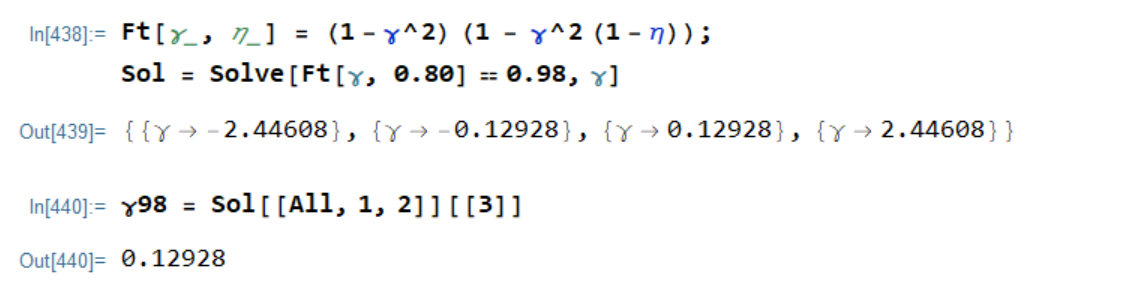
\includegraphics{./chapter_07/figs/Ftsolve.PNG}}

  \textcolor{midnightblue}{Like in introductory statistics problems, its helpful to think about the negative case: Given N sources with herald probability $p$, the probability of zero sources heralding is:}

  \textcolor{midnightblue}{

  $$P(\text{no herald}|N) = (1 - p_{binary}\left(\gamma, \eta\right))^N$$

  }

  \textcolor{midnightblue}{Then the probability of at least one herald is 1 minus the previous expression:}

  \textcolor{midnightblue}{

  $$P(\text{at least one herald}|N) = 1 - (1 - p_{binary}\left(\gamma, \eta\right))^N$$

  }

  \textcolor{midnightblue}{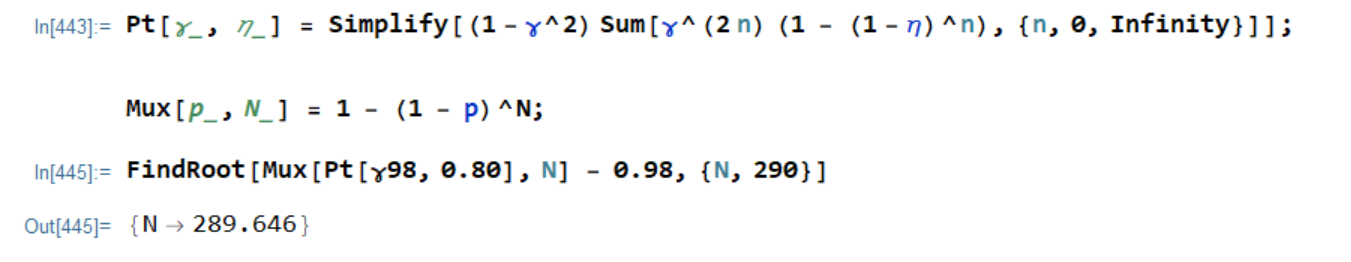
\includegraphics{./chapter_07/figs/mux_binary.PNG}}

  \textcolor{midnightblue}{About $\boxed{N = 290}$ sources are needed.}

  \textcolor{midnightblue}{3 pts for correct form of the multiplexing expression
  $P(\text{at least one herald}|N)$; 3 pts for similar number of sources $N$}
\end{enumerate}

A photon number resolving (PNR) SNSPD is able to discriminate the number of photons in a light pulse*. By heralding the idler mode with a PNR SNSPD, the generation of multi-photon signal pulses can be identified and discarded. There's a POVM for an ideal PNR single photon detector, where $i$ is the number of photons detected**:

$$\hat{\Pi}_{PNR}(i)=\sum_{n=i}^{\infty}\binom{n}{i}(1-\eta)^{n-i} \eta^{i}|n\rangle\langle n|$$

\begin{enumerate}
\def\labelenumi{\arabic{enumi}.}
\setcounter{enumi}{3}
\item
  (12 pts) Derive a herald probability $p_{PNR}$ and fidelity $F_{PNR}$ for the PNR POVM, following the steps in the previous sections with $i$ set to 1. You can use symbolic math tools to simplify them if you wish. The probability of successfully heralding states in the signal arm $p_{PNR}$ should now approach zero for $\gamma$ near one. Why is this?

  \textcolor{midnightblue}{ \textbf{Answer:} }
  \textcolor{midnightblue}{The POVM for one photon detected:}

  \textcolor{midnightblue}{

  $$\hat{\Pi}_{PNR}(1)=\sum_{n=1}^{\infty}n(1-\eta)^{n-1} \eta|n\rangle\langle n|$$

  }

  \textcolor{midnightblue}{First, derive the probability of getting a single photon detection from the PNR detector: $p_{PNR}(\gamma, \eta)$:}

  \textcolor{midnightblue}{

  $$\begin{aligned}
       p_{PNR}(\gamma, \eta) =\langle \psi | \Pi_{\text {PNR}} | \psi \rangle &= (1- \gamma^2) \sum_{\tilde{n}=0}^{\infty} \langle \tilde{n}_s \tilde{n}_i | \gamma^{\tilde{n}} \sum_{n=1}^{\infty}n(1-\eta)^{n-1} \eta|n\rangle\langle n| | n_s n_i \rangle \\
       \langle \psi | \Pi_{\text {PNR}} | \psi \rangle &= p_{PNR}\left(\gamma, \eta\right) =  \boxed{(1-\gamma^2) \sum_{n_s=0}^{\infty} \gamma^{2n_s} n_s(1-\eta)^{n_s-1}}\\
       p_{PNR}\left(\gamma, \eta\right) &=  \boxed{\frac{\gamma ^2 (1 - \gamma ^2) \eta }{(\gamma ^2 (\eta -1)+1)^2}}
   \end{aligned}$$

  }

  \textcolor{midnightblue}{Where either of the boxed answers are acceptable, and the last line was found using mathematica:}

  \textcolor{midnightblue}{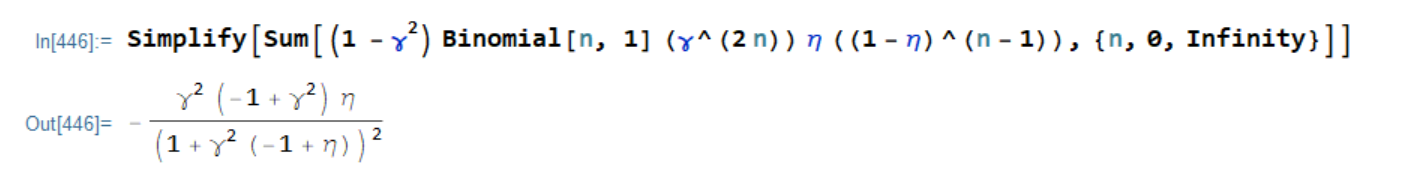
\includegraphics{./chapter_07/figs/simplify_ppnr.PNG}}

  \textcolor{darkred}{4 pts for $p_{PNR}\left(\gamma, \eta\right)$}

  \textcolor{midnightblue}{Second, derive the single photon fidelity, staring with the density matrix for the signal photon given a PNR herald event. Using (15) above for $\langle \psi | \Pi_{\text {PNR}} | \psi \rangle$ in the denominator helps simplify it significantly. }

  \textcolor{midnightblue}{

  $$\begin{aligned}
       \rho_s(\gamma,\eta) &= \frac{\operatorname{Tr}_i[\sum_{n=1}^{\infty} \gamma^{2n}n(1-\eta)^{n-1} \eta|n\rangle\langle n|n_s n_i \rangle \langle n_s n_i |]}
           {\langle \psi | \Pi_{\text {PNR}} | \psi \rangle}\\
           |1_s \rangle \langle 1_s | &= \frac{\cancel{(1 - \gamma^2)}(\gamma ^2 (\eta -1)+1)^2 \cancel{\gamma^2 \eta}}{\cancel{\gamma^2 \eta} \cancel{(1 - \gamma ^2)} }\\
           F_{PNR}(\gamma, \eta) &= \boxed{(\gamma ^2 (\eta -1)+1)^2}
   \end{aligned}$$

  }

  \textcolor{midnightblue}{4 pts for $F_{PNR}(\gamma, \eta)$}

  \textcolor{midnightblue}{For $\gamma$ near one, the SPDC is under strong pump power and is generating predominantly multi-pair states. A vanishing fraction of those states are single photon states that the PNR detector is able to distinguish and single-photon. Therefore, the PNR detector is signaling the generation of multi-pair states most of the time which should be discarded and do not contribute to $p_{PNR}$. For high efficiency $\eta$, only the vanishing single-pair creation rate contributes predominantly to $p_{PNR}$.}

  \textcolor{darkred}{4 pts for similar explanation}
\item
  (12 pts) Make a parametric plot for $0<\gamma<1$ with $F_{PNR}$ on the x-axis and $p_{PNR}$ on the y-axis. Plot the curve for a few different values of idler arm efficiency $0<\eta<1$. All curves should reach the same maximum herald probability. What is it?

  \textcolor{midnightblue}{ \textbf{Answer:} }
  \textcolor{midnightblue}{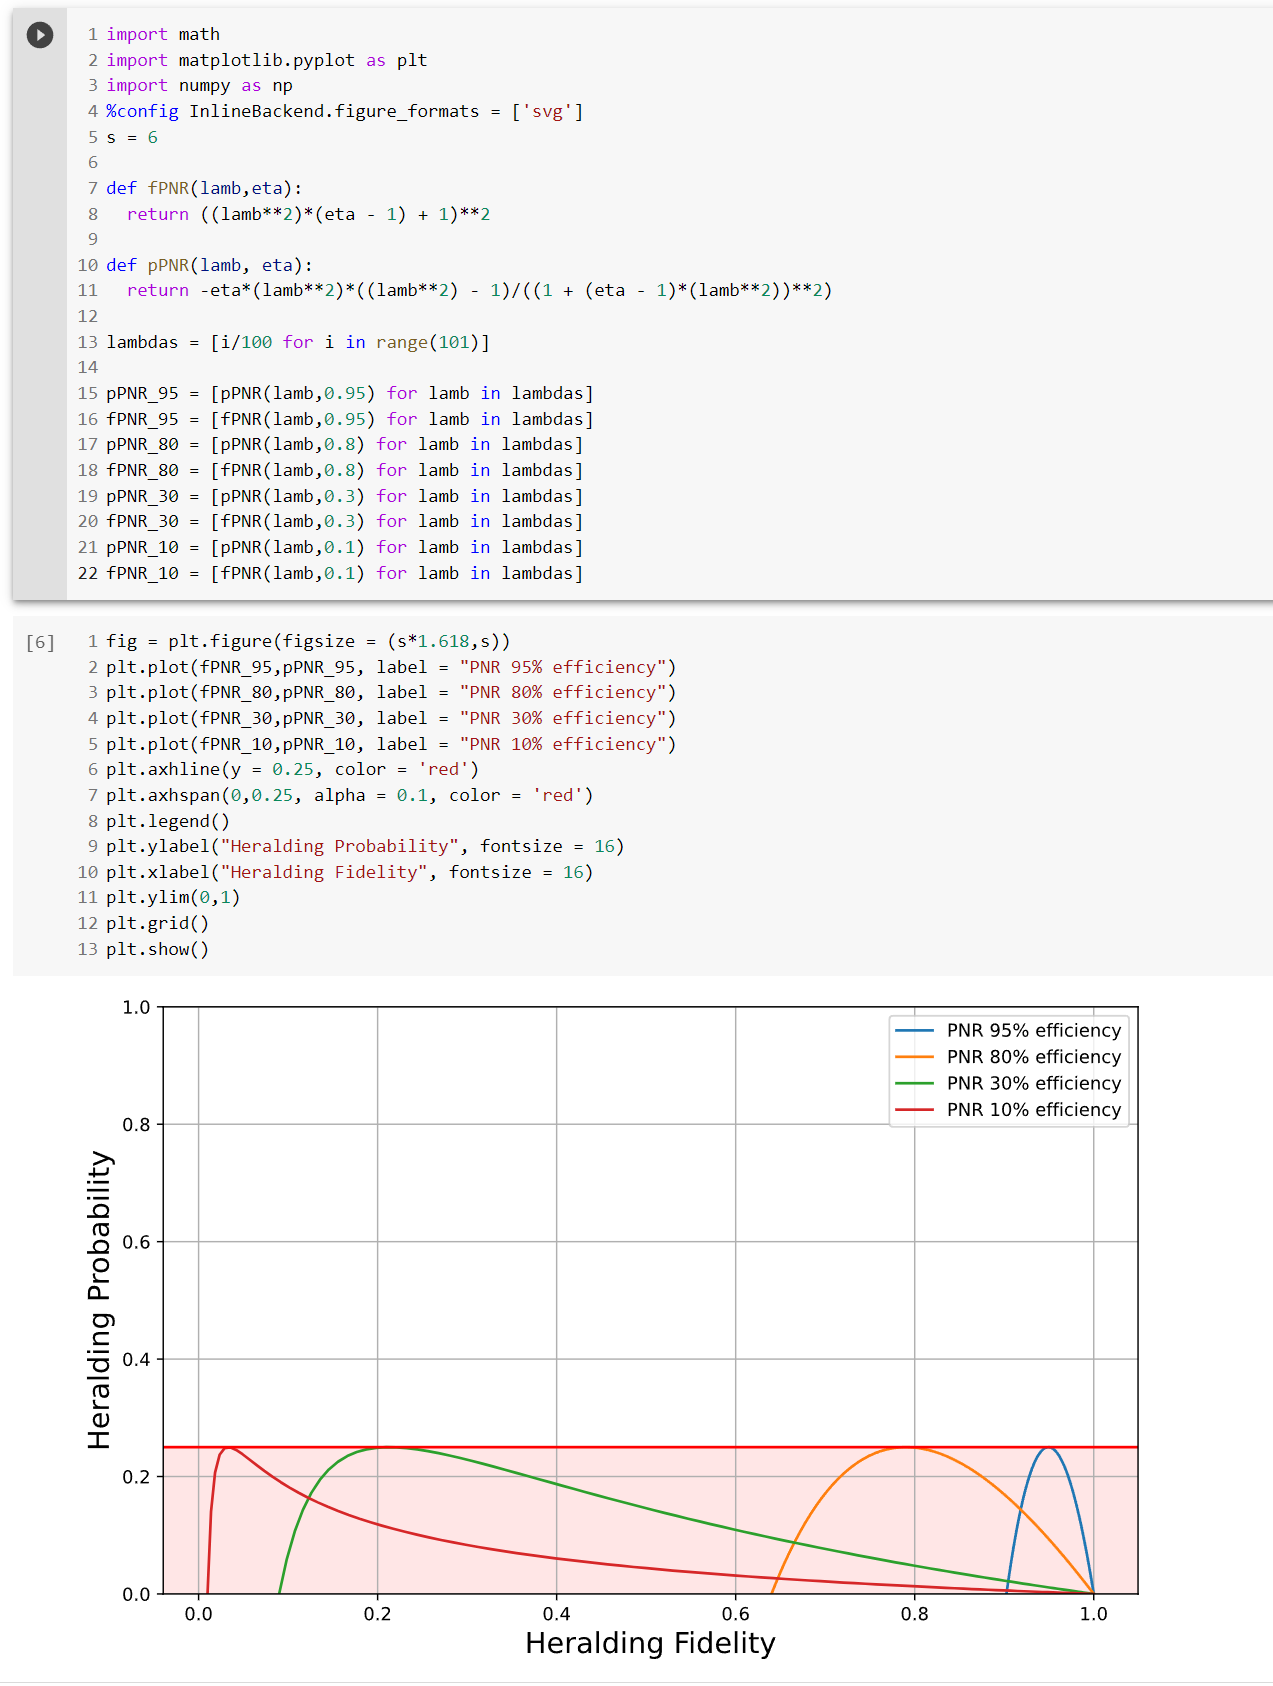
\includegraphics{./chapter_07/figs/PLT.PNG}}

  \textcolor{midnightblue}{ The the herald probability regardless of idler arm efficiency is 25\%. }

  \textcolor{darkred}{ 4 points for the 25\% limit; 8 points for a few plots at different $\eta$ }
\item
  (8 pts) Consider again the configuration in Fig.~\ref{fig:hsps} b. Find the number of sources using PNR detectors needed to reach 98\% single photon herald probability and fidelity with $\eta = 0.8$. Also find the number of sources for $\eta = 0.95$.

  \textcolor{midnightblue}{ \textbf{Answer:} }
  \textcolor{midnightblue}{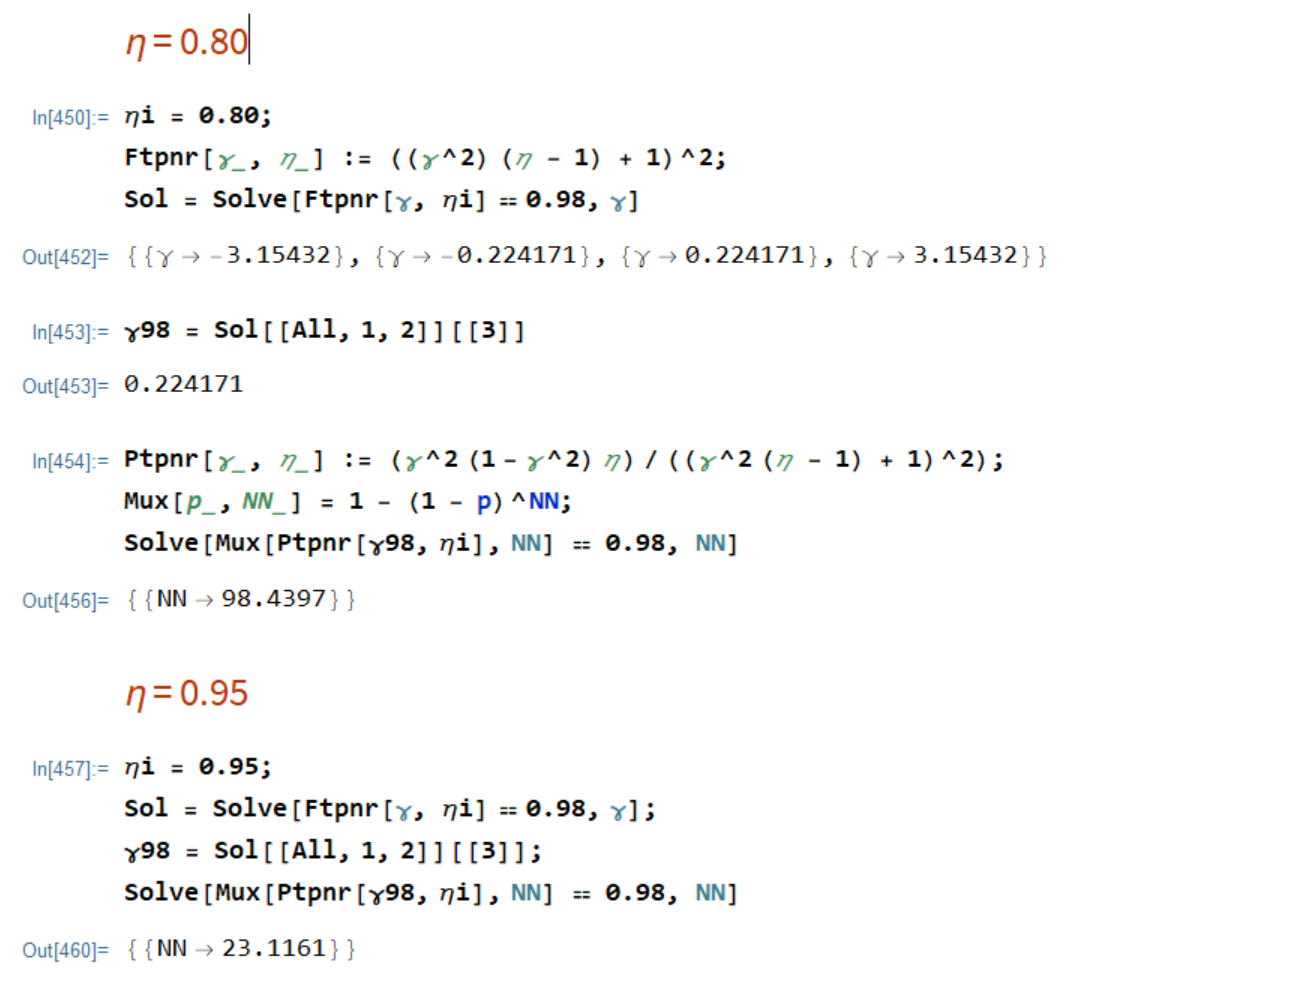
\includegraphics{./chapter_07/figs/pnrTotalPerf.PNG}}

  \textcolor{midnightblue}{About $\boxed{\text{98 sources are needed for the case with an 80\% heralding}}$, }

  \textcolor{midnightblue}{about $\boxed{\text{23 sources are needed with 95\% efficient heralding}}$}

  \textcolor{darkred}{ 4 points for each of the 2 answers. Answers that vary from these values by 2-3 sources are acceptable. }
\end{enumerate}

\hypertarget{software-tools}{%
\chapter{Software Tools}\label{software-tools}}

\hypertarget{software-tools-for-equipment-and-experiment-control}{%
\section{Software Tools for Equipment and Experiment Control}\label{software-tools-for-equipment-and-experiment-control}}

Much of my time during the phd was spent writing software. While the main product of a phd is papers and the underlying ideas of the experiments carried out, software was often used to rigorously encode these more semantic or ephemeral results. Sometimes, the efficacy of a certain excremental idea depends greatly on the simplicity and reliability of the software used to implement it. If the setup of an initially complex excremental arrangement -- for example the synchronization of intensity modulators and arbitrary waveform generator with a mode locked laser -- can be made significantly more simple through the use of software, then the idea becomes more practical and more likely to be adopted by other researchers.

For these reasons I include introductions to the software tools on which I spent the most time and gained the most benefit. Perhaps these repositories provide insight that the thesis so far has not.

\hypertarget{sequence-generator}{%
\section{Sequence Generator}\label{sequence-generator}}

The Sequence Generator repository is for generating AWG sequences that are synchronized with the Pritel OAC fast mode locked laser. This is needed for carving the mode locked laser signal with intensity modulators. This toolset was useful for my PPM project as well as a concurrent high rate QKD project with slightly different requirements.

The most important feature of this toolset is the ability to determine compatible AWG sample rates and sequence lengths for a given laser repetition rate, while imposing certain requirements, like that the AWG sequence length must be a multiple of 128 samples. The script supports situations where a small integer number of laser pulses does not math in time an integer number of AWG samples. The main requirement is that the time for the full AWG sequence to run must be an integer multiple of the laser repetition period, so that the AWG sequence can be repeated indefinitely without drifting out of sync with the laser.

The sections of code that undergo this analysis are located in the functions \texttt{determine\_ppm\_properties} and \texttt{determine\_regular\_properties} for the PPM and QKD applications respectively.

\href{https://github.com/sansseriff/sequence_generator/tree/main}{Sequence Generator Repository}

\hypertarget{section}{%
\section{}\label{section}}

\hypertarget{software-systems-and-operation}{%
\section{Software Systems and Operation}\label{software-systems-and-operation}}

\hypertarget{advanced-matplotlib-layouts-with-the-bisect-function}{%
\subsection{\texorpdfstring{Advanced Matplotlib Layouts with the \texttt{bisect()} function}{Advanced Matplotlib Layouts with the bisect() function}}\label{advanced-matplotlib-layouts-with-the-bisect-function}}

It can be difficult to create complex plot layouts with matplotlib, especially when the layout should have strict requirements, like neighboring axes that are aligned with one another. Before explaining a custom method for solving this problem through the use of a new function \texttt{bisect()}, its worth reviewing the more accepted methods of advanced matplotlib figure layout.

\hypertarget{subplot-mosaic}{%
\subsubsection{Subplot Mosaic}\label{subplot-mosaic}}

\href{https://matplotlib.org/stable/gallery/subplots_axes_and_figures/mosaic.html}{Subplot mosaic} is a tool for specifying the layout of a figure with a special python dictionary, demonstrated by this example from the docs:

\begin{minted}
[
frame=lines,
framesep=2mm,
baselinestretch=1,
bgcolor=extralightgray,
fontsize=\footnotesize,
linenos]
{python}
fig = plt.figure(layout="constrained")
ax_dict = fig.subplot_mosaic(
    [
        ["bar", "plot"],
        ["hist", "image"],
    ],
)
ax_dict["bar"].bar(["a", "b", "c"], [5, 7, 9])
ax_dict["plot"].plot([1, 2, 3])
ax_dict["hist"].hist(hist_data)
ax_dict["image"].imshow([[1, 2], [2, 1]])
identify_axes(ax_dict)
\end{minted}

\includegraphics{./chapter_08/figs/sphx_glr_mosaic_001_2_0x.webp}

There are methods of changing the aspect ratios of the plots, but tools for imposing alignment constraints across plots are limited. For example, notice in the example above how the (1,1) plot axes are not vertically aligned with the (0,1) plot above.

\hypertarget{gridspec}{%
\subsubsection{Gridspec}\label{gridspec}}

\href{https://matplotlib.org/stable/gallery/lines_bars_and_markers/scatter_hist.html\#sphx-glr-gallery-lines-bars-and-markers-scatter-hist-py}{Gridspec} is a tool for more carefully specifying a grid layout. Space between plots can be specified, and the relative widths or heights of columns and rows can be customized. Gridspec offers a lot of control, but it requires many custom parameters that can be unintuitive to derive.

\hypertarget{add_axes}{%
\subsubsection{Add\_axes}\label{add_axes}}

One of the simplest ways of adding subplots to a figure is with the \texttt{fig.add\_axese(rect)} method. The \texttt{rect\ =\ {[}ll\_x,\ ll\_y,\ width,\ height{]}} specifies the x and y coordinate of the lower left corner with the first two parameters, and the width and height with the second 2 parameters. Multiple uses of \texttt{add\_axese()} offers maximum control for creating advanced layouts, but specifying all the correct \texttt{rect} arrays can get very confusing. Figure Fig.~\ref{fig:layout_sketch} illustrates the types of calculations that become necessary when the specific location and size of each subplot must be specified under certain constraints.

\hypertarget{fig:layout_sketch}{%
\begin{figure}
\centering
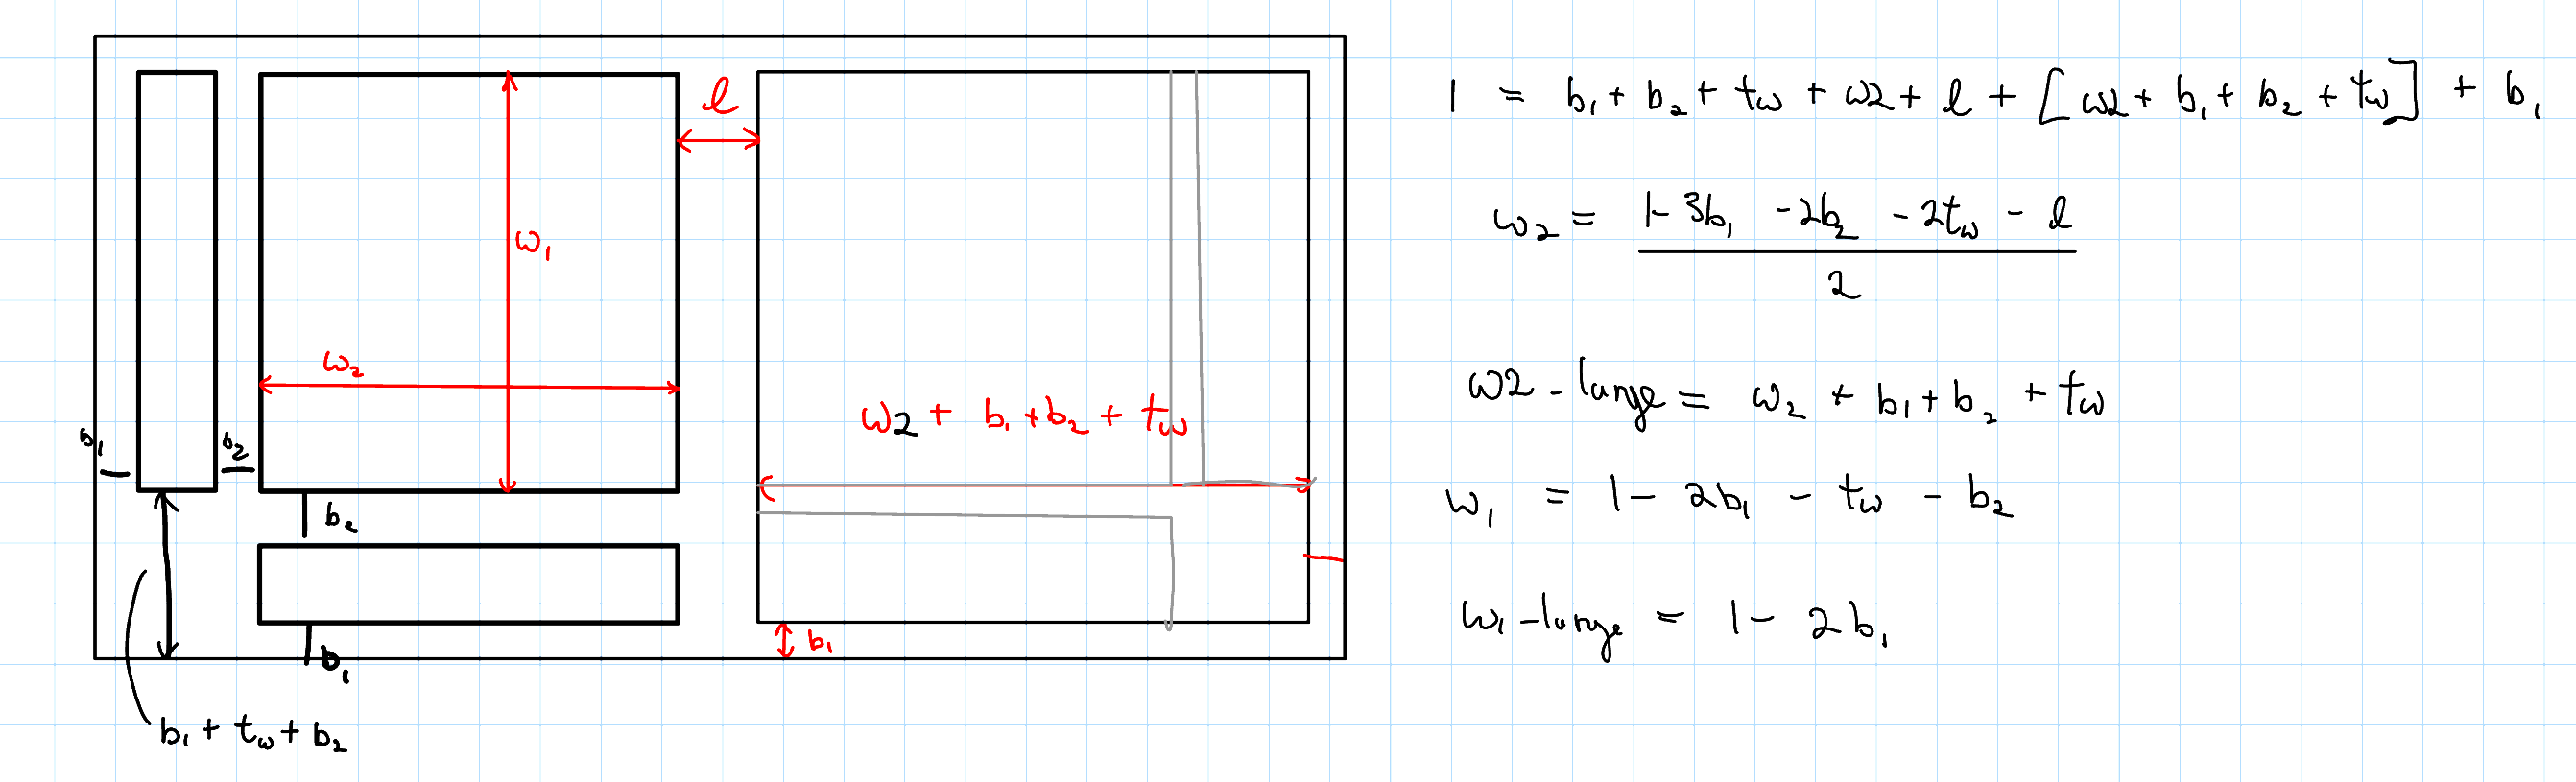
\includegraphics{./chapter_08/figs/layout_sketch.png}
\caption[{Rough sketch for layout with add\_axese()}]{\textbf{Sketch for layout with add\_axese().}}
\label{fig:layout_sketch}
\end{figure}
}

\hypertarget{bisect-method}{%
\subsubsection{\texorpdfstring{\texttt{bisect()} method}{bisect() method}}\label{bisect-method}}

\hypertarget{how-a-sorption-fridge-works}{%
\section{How A Sorption Fridge Works}\label{how-a-sorption-fridge-works}}

to put something only in the mkdocs/html output:

to put something only in the latex output:

You can do footnotes like this\footnote{This is a footnote}

use \boldsymbol for bold latex:

\textbf{Fidelity and Rates vs $\boldsymbol \mu$}

Here are a few bold characters together: $\boldsymbol{\mu \quad \beta \quad \gamma}$

For units, use \mathrm{nm}:
This is a number with units: $138.3~\mathrm{nm}$

Refer to a figure with Fig.~\ref{fig:figurename} or Fig.~\ref{fig:figurename} or for multiple Fig.~\ref{fig:figurename}

Until I figure something more shorthand, you can set colors with ``\textless span\textgreater{}'' tags:

\textcolor{midnightblue}{ This text is blue. And it changes lightness when darkmode is witched }

\hypertarget{fig:figurename}{%
\begin{figure}
\centering
\includegraphics[width=0.7\textwidth,height=\textheight]{./chapter_08/figs_06/fig1b_light.svg}
\caption[{Figure label for in thesis index here.}]{\textbf{Caption title here} a) Long caption here}
\label{fig:figurename}
\end{figure}
}

\hypertarget{fig:figurename2}{%
\begin{figure}
\centering
\includegraphics[width=0.7\textwidth,height=\textheight]{./chapter_08/figs_06/hsps_light.svg}
\caption[{Figure label for in thesis index here.}]{\textbf{Caption title here} a) Long caption here}
\label{fig:figurename2}
\end{figure}
}

to have a ``~'' space in latex and a no break space in html\ldots{} ``\&\#160'', just use ``~''. That's a forward slash and a space.

The formatting of multi-line divs is very important. This will render correctly:

{\color{midnightblue} 

$$math stuff 1$$

}

But this won't:

{\color{midnightblue} 

\begin{minted}
[
frame=lines,
framesep=2mm,
baselinestretch=1,
bgcolor=extralightgray,
fontsize=\footnotesize,
linenos]
{nil}
$$math stuff 2$$
\end{minted}

}

And this won't

\begin{minted}
[
frame=lines,
framesep=2mm,
baselinestretch=1,
bgcolor=extralightgray,
fontsize=\footnotesize,
linenos]
{nil}
$$math stuff 3$$

</div>
\end{minted}

the file where you're working on bokeh styling is at :

C:\Users\Andrew\OneDrive - California Institute of Technology\JPL.Jitterate\peacoq\src\bokeh\_hists\_js\_callbacks.ipynb

\printbibliography
\end{document}
